% Review Christian Stary January 2020

\chapter{Aspects for further standardisation activities}

CS: Hochkommas und - im pdf falsch gedruckt.

In this chapterr various aspects of the subject oriented modelling and programming concept are outlined. These aspects have already been published on different conferences. The following sections are based on these publications. CS: They contain original text parts and thus, the conclusions need to be aligned to the standardization effor, as tried for Fog Computing.
The concepts described in theses sections will be part of future standardisation activities.
The following sections are based on following publications:\\
\begin{list}{-}
	\item Subjects and Shared Input Pools:
	\item Hierarchies in Communication Oriented Business Process Models:
	\item Business Activity Monitoring for S-BPM: \cite{article:SubProcessMon}
	\item Subject Oriented Project Management:
	\item Subject-oriented Fog Computing: \cite{article:FogComp}
	\item Activity based Costing \cite{article:SBPMCosting}
\end{list}

\section{Subjects and Shared Input Pools}

Shared input pools have the same structure like subject-specific ones, and thus, the same properties like the standard input pool. The only difference is that different subjects can deposit in or remove messages from a shared input pool. Subjects that want to send a message via a shared input pool do not use a subject name as addressee of a message, but the name of a shared input pool instead. In a distributed system several shared input pools for different purposes can be used. Figure 7 shows the slightly changed structure of the traffic management system when operating it with a shared input pool CS: hier fehlt das originäre Beispiel als Bezugspunkt. The subject "Car detection" represents the shared input pool.


\begin{figure}[htbp]
	\centering
	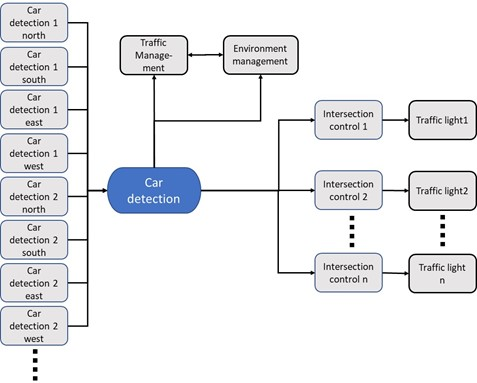
\includegraphics[width=0.7\linewidth]{Figures/Chapter5/figuresshared/SharedInputPoolExample.jpg}
	\caption[Traffic Management System with Shared Input Pool]{Traffic Management System with Shared Input Pool}
	\label{fig:SharedInputPooTraffic}
\end{figure}


Shared input pools make a distributed system more flexible when additional participants or nodes are added. For instance, a third intersection control could be added to the traffic management system without much effort. In this case, only the additional detectors and the components for controlling the intersection have to be complemented and linked to the shared input pool. The extension would have no impact on the behavior of the other subjects and their behavior in that system.
There is one additional attribute for shared input pool: It defines whether a message will be removed from the input pool once a message has been picked up by a receiving subject. This mechanism is required, since several subject may need to process a particular message. In addition, it allows keeping historical information in the input pool, in particular for analyzing the content of an input pool independently of the behavior of interacting subjects. 
The messages of an input pool can be analyzed with respect to certain patterns of its messages. In order to perform such an analysis, Complex Event Processing (CEP) concepts can be applied. Complex Event Processing can be encapsulated in a subject. A subject of this kind scans the messages of a shared input pool and checks whether patterns of interest can be found. Once such a pattern is identified, a message including the discovered pattern can be sent to other participants, and initiate further activities. Figure 8 shows the traffic management example enriched with subjects processing complex events.
In the example, the subject "CEP pollution analyzer" can analyze the time between cars passing the intersection in a certain time period. It can identify the events "low traffic" or "high traffic" and send it to the subject "Environment management". In case of tunnels, the subject "Environment management" might react to this information in a different way compared to open air settings. 


\begin{figure}[htbp]
	\centering
	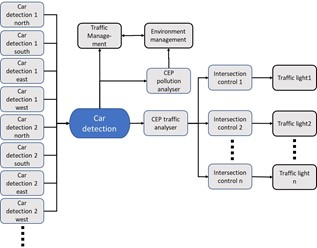
\includegraphics[width=0.7\linewidth]{Figures/Chapter5/figuresshared/SharedInputPoolEvent.jpg}
	\caption[Shared Input Pools and Complex Event Processing]{Shared Input Pools and Complex Event Processing}
	\label{fig:sharedInputPoolEvents}
\end{figure}

\subsection{Implementing Shared Input Pools}
As mentioned earlier, shared data repositories represent a single point of failure of a distributed system. A malfunction of a shared data storage component or device may have a significant impact on the functionality of the whole distributed system. If a subject or a communication line is disturbed, only a small part of a system may be concerned but if a shared data store is down this has an impact on all subjects accessing this input pool.
\\
In addition to this operational problem it must be decided in the course of organizational implementation which organization is held responsible for running and maintaining the system hosting the shared data. Such issues become prominent, if a distributed system is connecting several independent organizations, e.g., different companies in a supply chain. Distributed systems run by independent organizations may also have to deal with several changes dynamically, affecting the data quality and system stability. Even companies can be replaced by other organizations. If only functional subjects are concerned, such a change can be managed without affecting the operation of the entire system: The execution of a subject is just assigned to the new actor. The problem is more serious if a company leaving a distributed system is responsible for running the system with shared data, as other participants of the shared system are affected. Then, a new company still part of the distributed system must take over the responsibility for the shared data. The migration of these data from one company to another can become very cumbersome from the business point of view and from a technological perspective, too.
One way to solve these problems is implementing shared input pools with blockchain technology. A blockchain is an open, distributed ledger that can record transactions efficiently in a verifiable and permanent way. Blockchains allow to achieve the integrity of a collection of data in a distributed peer-to-peer system, whereas the number of the peers is unknown and an unknown number of them are not reliable and trustworthy \cite{book:Blockchainbasics}. 
\\
Today, blockchains are mainly used for managing the ownership of money, goods, real estates, etc. Each participant in a distributed system may have a copy of a blockchain. Changes in a blockchain follow a mechanism which manage changes in a consistent way and the change protocol guarantees that any participant will have again a consistent copy after a change. A change of a blockchain means that a new data record is added, and nothing can be removed from a block chain. Adding a new block to a block chain requires some effort from parties involved in a blockchain. This effort is rewarded by adding crypto money to the party when having accomplished the task successfully. These rewards serve as an incentive for the creators of blocks. 
\\
Although heavily questioned with respect to effort and gains by practitioners \cite{article:BlockchainUniverse} blockchain technology provides concepts ensuring the trustworthiness of system components. The latter becomes crucial when operating sensitive distributed systems, such as public transportation and healthcare, in particular when event-based data fusion is needed, where nodes of various type (sensor systems, vendor-specific monitoring systems. user devices, household items, etc.) exchange notifications of events and decision-relevant data with each other. In such settings, not only notification mechanisms needs to be streamlined in case of heterogeneity of nodes, but also data source trust is important for further processing and system behavior \cite{article:EventbasedSensor}.
\\ 
In order to ensure dependable sharing of data, these basic properties of blockchains need to be adapted to the requirements of a shared input pool. Hence, a blockchain-oriented implementation of a shared input pool must meet several requirements:
\begin{enumerate}
	\item Subjects can subscribe for the access to a shared input pool.
	\item Subjects subscribed for an input pool may deposit or read events from that input pool. 
	\item Events can be marked as removed from a shared input pool.
	\item Subjects may analyze the content of a blockchain, e.g., when processing complex events.
	\item There must be a mechanism that a block chain can be deleted, once all involved parties agree on that.
\end{enumerate}

Traditionally data received from "things" are not very complex. These data are mainly values as measured by sensors, or binary signals. This may lead to a paradox situation: If such simple data are to be stored in a blockchain, the fee to be paid for adding blocks containing simple data is larger than the value being transferred. 
One way to solve the resulting incentive problem is to use permissioned block chains instead of open block chains: Blockchains for dedicated distributed application are not open blockchains like the ones implementing the management of digital currencies. 
\\
For the implementation of shared input pools, we suggest managed or permissioned blockchains. For instance, Hyperledger Fabric \cite{article:hyperledger} is an open source implementation of a permissioned blockchain. Unlike to a public permissionless network, the participants are known to each other, rather than staying anonymous and interacting untrusted. It means, while the participants may not fully trust one another, e.g., in case of being competitors in the same industry sector, a network can be operated under a governance model that is built on the extent of trust existing between participants, such as a legal agreement or framework for handling disputes. When building a business process with known participants, such type of a blockchain implementation would be sufficient. Consensus algorithms for permissioned blockchains are faster and do need much less energy than permissionless blockchain networks. 
\\
In \cite{article:Blockbench} it is reported that hyperledger fabric is the fastest available permissioned blockchain. The transaction throughput could even be increased from 3,000 to 20,000 transactions per second \cite{article:hyperledgerfabric}.
\\
When using Hyperledger to create blockchain networks of that kind, a hyperledger blockchain network provides a technical infrastructure offering ledger and smart contract (chaincode) services to applications. Primarily, smart contracts are used to generate transactions which are subsequently distributed to each peer node in the network where they are immutably recorded on their copy of the ledger. The users of applications can be users of client applications or blockchain network administrators.
\\
Subject add messages to the shared input pool and other subjects want to read these messages. If a shared input pool is implemented as a blockchain it is necessary that the chain code (smart contract in Ethereum) realizing the functions of the shared input pool must interact with the world outside the block chain. In hyper ledger fabric (including Ethereum), this problem is solved by so called oracles. We suggest using the blockchain patterns Oracle and Reverse Oracle as described in \cite{book:Blockchainapplications}. For flexibility reasons we prefer off chain oracles - see figure \ref{fig:sharedblockchain}.



\begin{figure}[htbp]
	\centering
	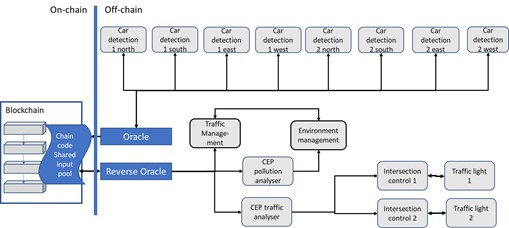
\includegraphics[width=0.7\linewidth]{Figures/Chapter5/figuresshared/Block-Chain.jpg}
	\caption[Utilizing block chain patterns Oracle and Reverse Oracle]{Utilizing block chain patterns Oracle and Reverse Oracle}
	\label{fig:sharedblockchain}
\end{figure}

\subsection {Conclusion}
The more the Internet of Things (IoT) propagates into domain-specific applications, the more stakeholders get involved with respect to business and user requirements. They expect omnipresent use and adaptation on demand. Ensuring robust and semantically correct operation in dynamically networked IoT environments requires tools and development methods to handle complex patterns of interactions due to the different components and capabilities of actors.\\
These patterns refer to the (reactive) flow of control and correct exchange of data. We have proposed an integrated approach based on subject-oriented process models. These role-specific representations allow behavior abstractions on various levels of granularity and can be enriched with a mechanism for handling complex events and sharing data. The data handling mechanism is bound to exchanging messages and a blackboard-like structure. Its behavior can be implemented through blockchain technologies, in case a single point of failure in system operation should be inhibited. The latter is of crucial importance, once the data exchange between IoT-system elements should be trustworthy and traceable.\\
The presented approach should facilitate transparent development and stakeholder understanding of (complex) IoT systems in dynamic settings, due to the implementation-independent representation on a mainly diagrammatic level based on a minimalistic notation, stemming from subject-oriented modeling. Abstractions and decomposition into IoT system components encapsulate behavior. The overall behavior of an IoT system is determined by a set of interactions that integrates the control flow with data exchange patterns from a semantic process perspective. Application design can be understood as top-down approach with the functionality specific to the IoT application residing on an edge operating system. Platform services implement all functional requirements, and are backed by communication and information processing technologies. Cross-functional issues, such as secure operation, business-relevant standardization, and critical event handling can be explicated on an implementation-independent level due to the semantic process representation scheme. The resulting models are executable and thus, can be adapted dynamically.


\subsection{Future Work}
Due to the novel conceptual integration addressed, several aspects and topics need to be addressed by future research:
\begin{list}{-}{spacing}
\item From an application perspective, the results need to be aligned with novel industry 4.0 concepts (cf. [29]), since there not only existing standards are framed by business processes, but also distributed operation of production-relevant processes and real-time sharing of data.
\item From an implementation perspective, our approach requires a (prototypical) realization of an appropriate block chain mechanism for managing shared input pools meeting all requirements in section 4.
\item From an industry perspective, performance evaluations might lead to reconsider our conceptual findings, e.g., how to manage a shared input pool of a distributed system in real time.
\item Definition of structural semantics in OWL
\item Definition of execution semantics in ASM
\end{list}

\section{Hierarchies in Communication Oriented Business Process Models}
PASS  offers powerful possibilities for structuring complex process systems. The ways to do that are demonstrated with an example.
As an example we will consider a process for realizing a car break down service. This service consists of several connected processes. There is the main process for handling the car accident and supporting e.g. processes for organising towing and repair shop services. Insurance companies may be involved for covering damages, the customer gets an invoice, uses money transfer services or banks for paying the invoice. These processes are executed by various organisations like help desk service companies, towing service companies, car repair workshops banks etc.. In most business process projects not all parts of processes are described in detail. Only a certain part is considered, e.g. only the help desk process has to be considered in detail. In order to do so we have to consider the whole environment in which a considered process is embedded. We have to know which relations exists to these other processes. It is necessary to know which inputs are rquired by neighbour processes and which results they deliver. A help desk process which organizes the towing services has to know how the towing service is requested and which further interactions are required. For instance it must be agreed whether the towing service informs the client about the arrival time of the towing truck or the help desk does it.


\subsection{Process Architecture}

Rectangles represent processes. Each process has a name. Processes consists of other processes and/or subjects. The lines between the rectangles represent the communication channels between processes. Each communication channel has a nameand can contain other communication chan-nels and/or messages.

Figure \ref{fig:car-service-level1} shows the highest process level of the car break down service. In the "car use" process the event "car break down" happens. In order to organize support an interaction is initiated with process "car break down service" . Between these processes messages are exchanged which are elements of the communication channel "Car break down handling".\\


\begin{figure}[htbp]
	\centering
	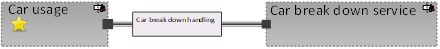
\includegraphics[width=0.7\linewidth]{Figures/Chapter5/figures-hierarchy/Car-Service-Level1.jpg}
	\caption[High level structure of car break down service]{High level structure of car break down service}
	\label{fig:car-service-level1}
\end{figure}



Figure \ref{fig:car-service-leve2} shows the next process structure level of the process "car break down ser-vice". In this level the process "Car break down service" is spltid in 10 processes. The processes "Bank", "Insurance service", "Car repair workshop", "Incident Management","Mobility Manage-ment" and "Towing Management" have a communication channel to the prcess "Car usage". This means the communication channel "Car break down handling" is split into five communica-tion channels. Each of them covers the communication with the relared process, e.g. the communi-cation channel "Accident notification Car break down" is the communication channel between the processes "Car usage" and "Incident Management".\\


\begin{figure*}[htbp]
	\centering
	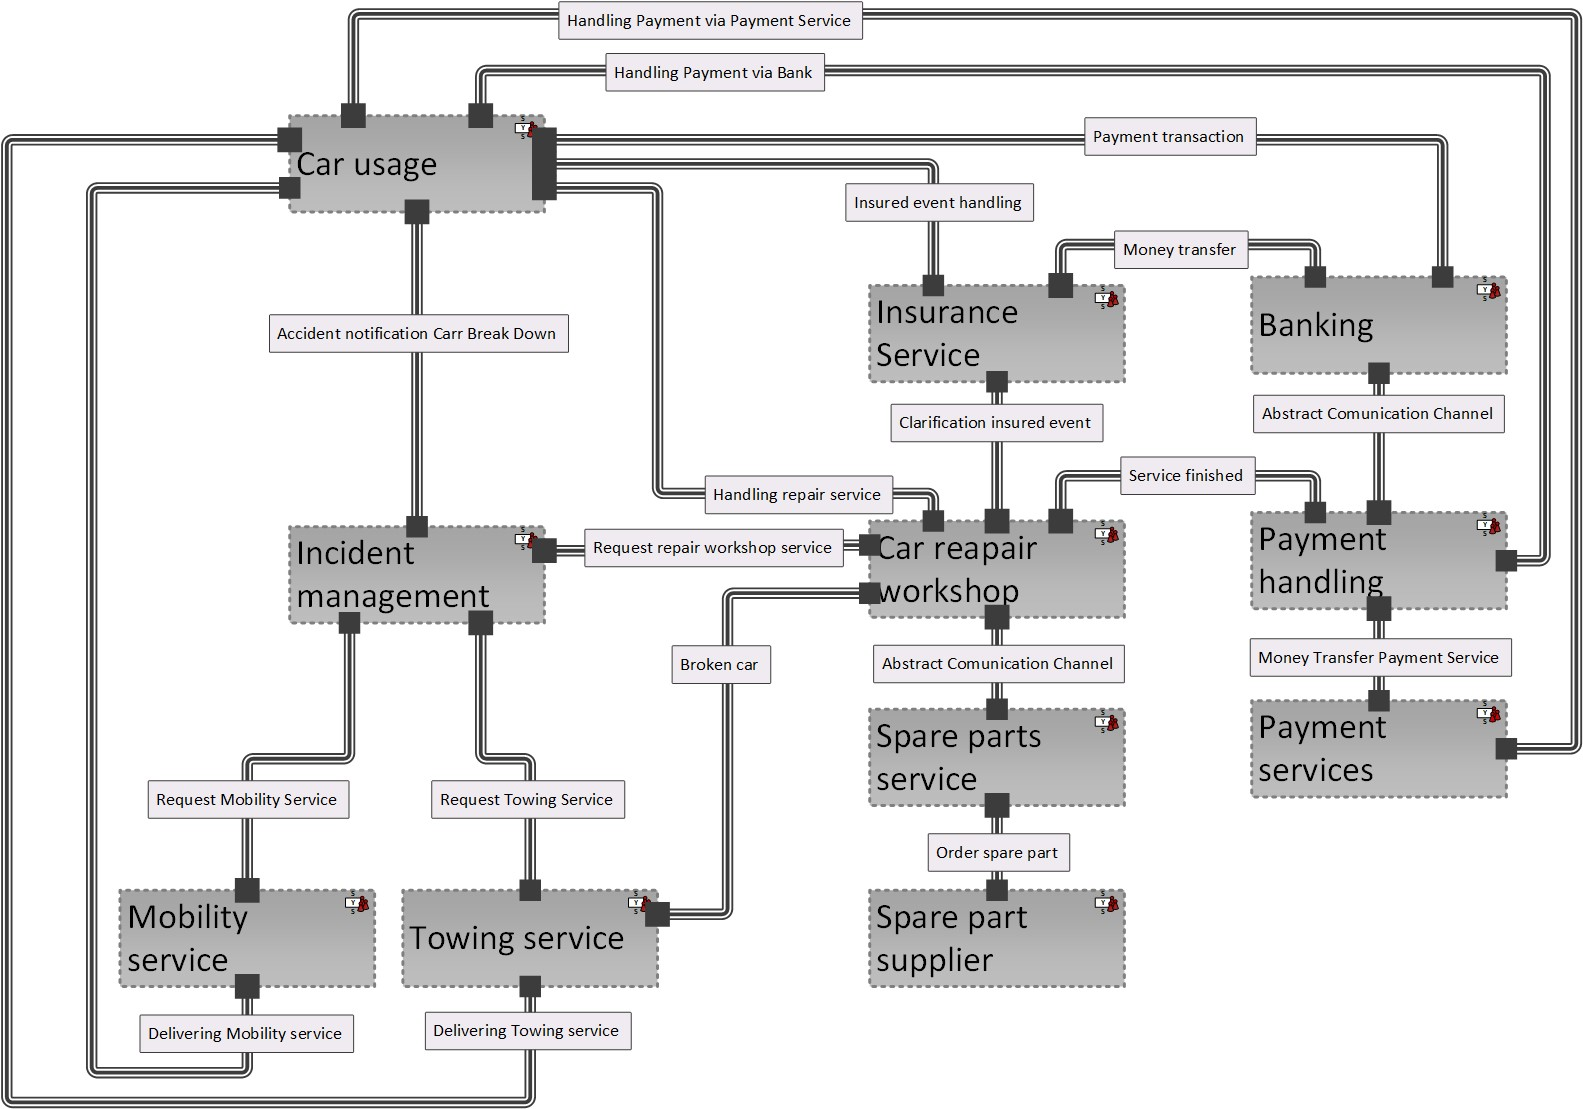
\includegraphics[width=0.8\linewidth]{Figures/Chapter5/figures-hierarchy/Car-Service-Leve2}
	\caption[Structure of the Emmergency Call Handling Process]{Structure of the Emmergency Call Handling Process}
	\label{fig:car-service-leve2}
\end{figure*}



Inside a process there can be also processes. This means that levels of processes can be built. Figure \ref{fig:car-service-lev3} shows the next deeper level of our process hierarchy. The process "Car repair workshop" is structured in six processes. According to this separation the communication sets are also splitted e.g. the communication set "Handling repair service" is splitted into three parts, one part is han-dled by the process "Service scheduling" the other by the process "Car droping" and the third one by the process "Customer Satisfaction".\\

\begin{figure*}[htbp]
	\centering
	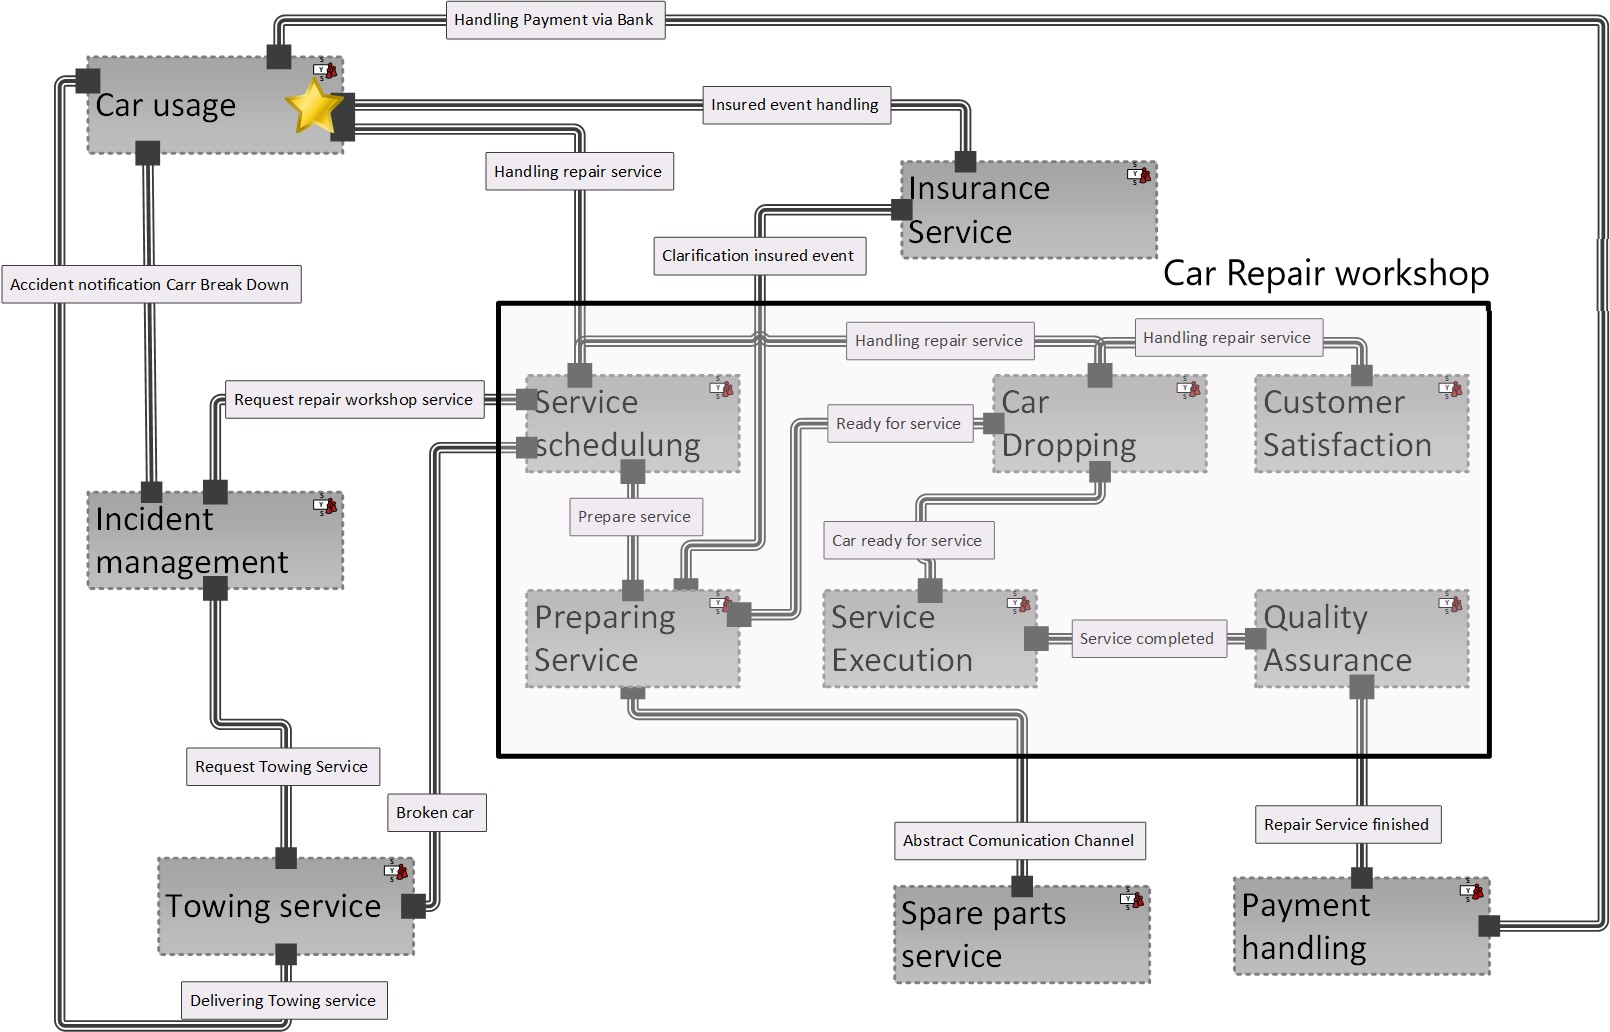
\includegraphics[width=0.8\linewidth]{Figures/Chapter5/figures-hierarchy/Car-Service-Lev3}
	\caption[Details of the "Car repair workshop" Process]{Details of the "Car repair workshop" Process}
	\label{fig:car-service-lev3}
\end{figure*}

As already mentioned, processes cannot communicate directly with each other. The active entities of a process, the subjects communicate with each other. This means messages from one process are sent to an other process are reveived by a subject inside of that process. Messages belonging to a channel are assigned to a sending or receiving subject at the lowest level of a process architecture. This lowest level of a process description is the subject interaction diagram (SID) which shows the involved subjects of a process and the messages they exchange. In the following we consider the process incident management in more detail. This process does not contain other processes like the process "Car Repair Shop". The process "Incident management" contains a Subject Interaction Diagram. Some of the subjects of a process communicate with subjects in other processes. These subjects are called border subjects because they are at the border of a process to other prcesses. Figure \ref{fig:car-service-lev4} shows the process "Incident management" with its border subjects. There is a border subject "Help agent" which communicates with the processes "Towing service", "Mobility ser-vice"and  "Car repair workshop", precisely it communicates with a subject in one of these processes. Another border subject of the process "Incident management" which is called "Help desk"communicates with the process "Car usage".\\

\begin{figure}[htbp]
	\centering
	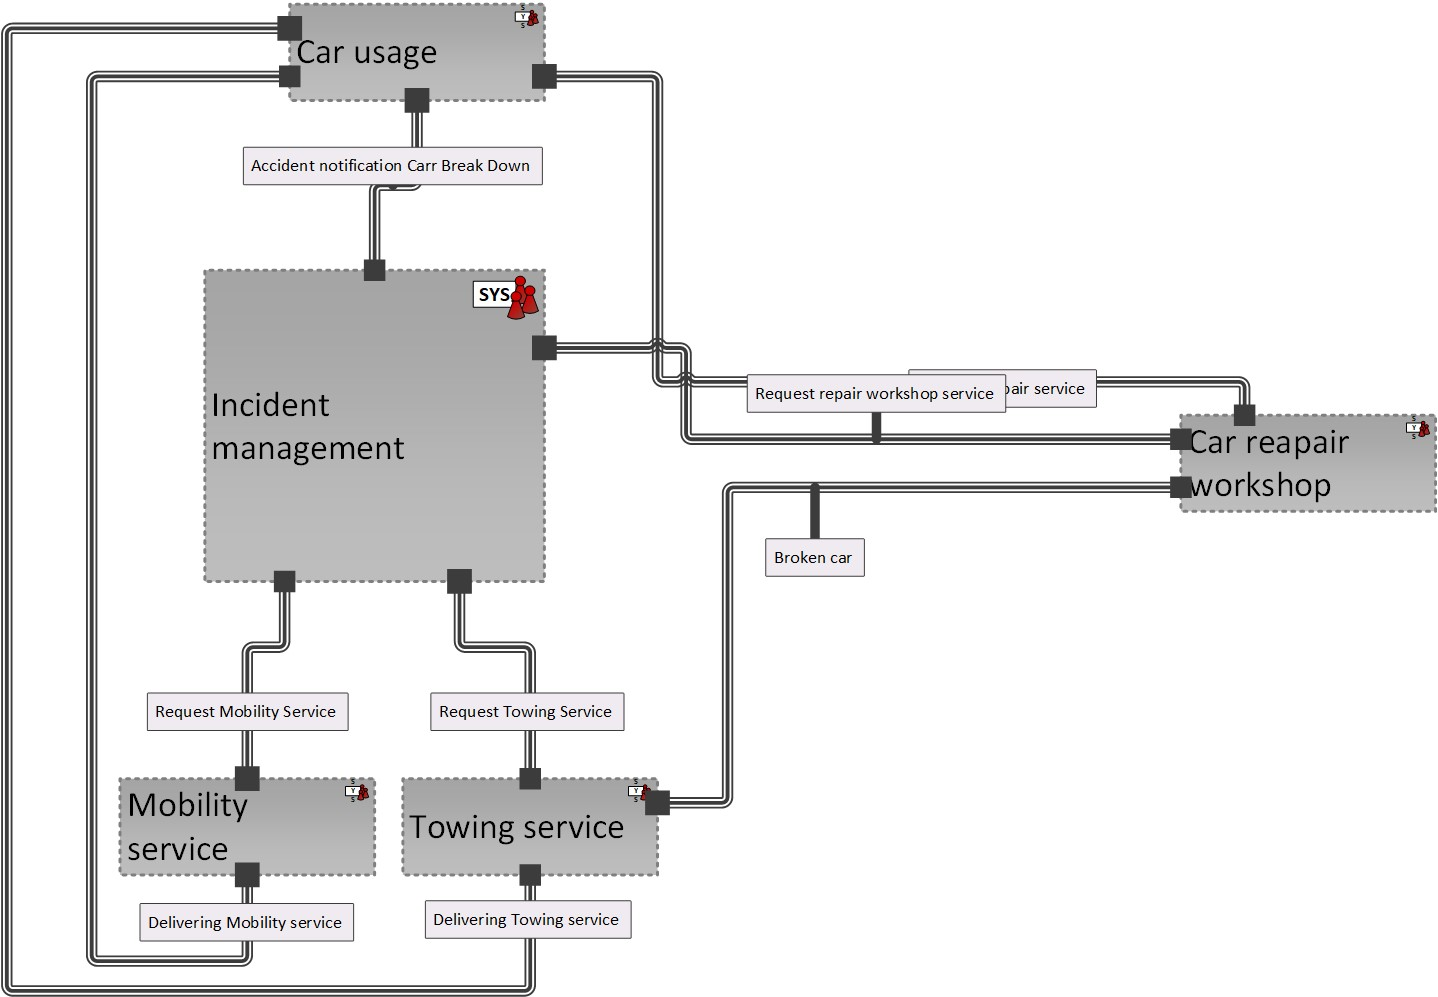
\includegraphics[width=0.9\linewidth]{Figures/Chapter5/figures-hierarchy/Car-Service-Lev4}
	\caption[Neighbors of the "Incident Manaement Process"]{Neighbors of the "Incident Manaement Process"}
	\label{fig:car-service-lev4}
\end{figure}

The border subjects of the process "Incident management" must have a coresponding border sub-ject at the neighbour processes. The border subjects "Call agent" communicates with the border subject "Help requestor" of process "Car usage" and the border subject "Help agent" communi-cates with border subjects of the processes "Car repair workshop", "Towing service and "Mobility service". The process "Incident management" with all the border subjects is shown in  figure \ref{fig:car-service-lev5}.\\

\begin{figure}[htbp]
	\centering
	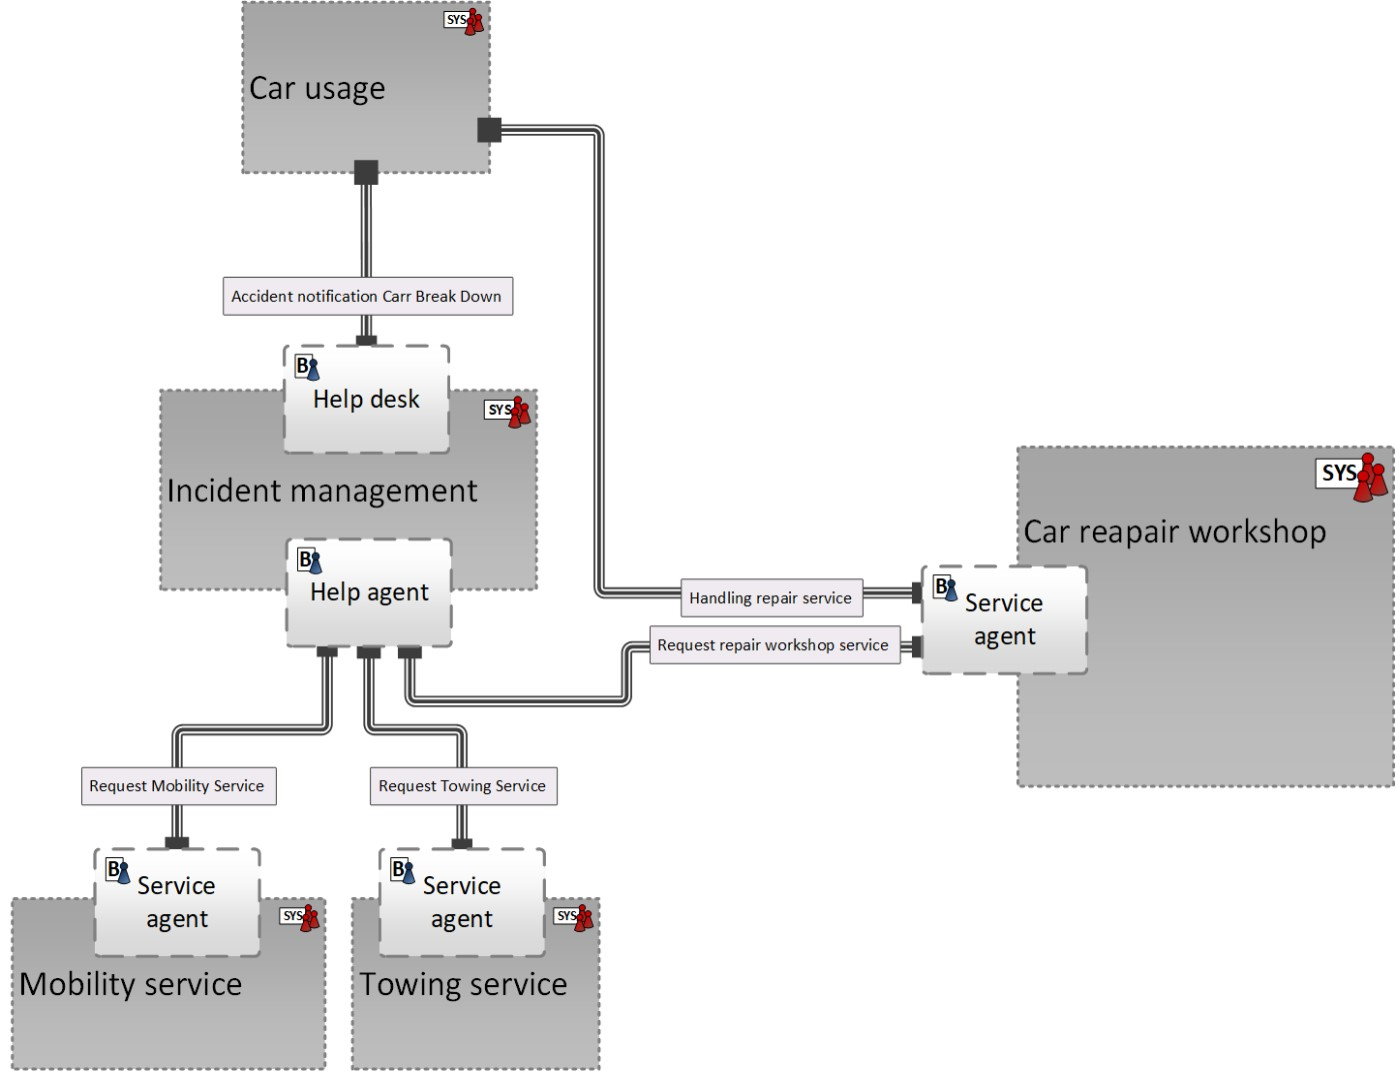
\includegraphics[width=0.9\linewidth]{Figures/Chapter5/figures-hierarchy/Car-Service-Lev5}
	\caption[Border subjects of the "Incident Management" Process]{Border subjects of the "Incident Management" Process}
	\label{fig:car-service-lev5}
\end{figure}

The border subjects of the processes "Mobility service", "Towing service" and "Car repair work-shop" have the same name “Service agent” but these are different subjets because they belong to different processes. Because the process "Car repair workshop" consists of several layers the corre-sponding border subject can be in a process which is part of process "Car repair workshop" in a lower level.\\
From the perspective of the subjects inside of the process "Incident managent" are the border subjects of the processes "Mobility service", "Towing service" and "Car repair workshop" interfaces to these processes, therefore they are called interface subjects in the Subject Interaction Diegram of a process. Figure \ref{fig:car-service-lev6}shows the Subject Interaction Diagram of the process incident management.\\


\subsection{Behavioral Interface}
Processes to which a considered process has communication relationships are called process neighbours or for short neighbours. Now we want to consider the details of the communication relationships between two neighbours. The interface between two processes is defined by the related border subjects and the allowed sequences in which the messages are exchanged between them in a communication channel. As already described above each message is defined by a name and the data which are transported the so-called payload. A border subject observes the behavior of the border subject of the neighbour process and vice versa. Figure \ref{fig:car-service-lev8} shows the border subject "Help desk" of the processes "Incident Management" which communicates with the border subject of process "Car usage".\\

\begin{figure}[htbp]
	\centering
	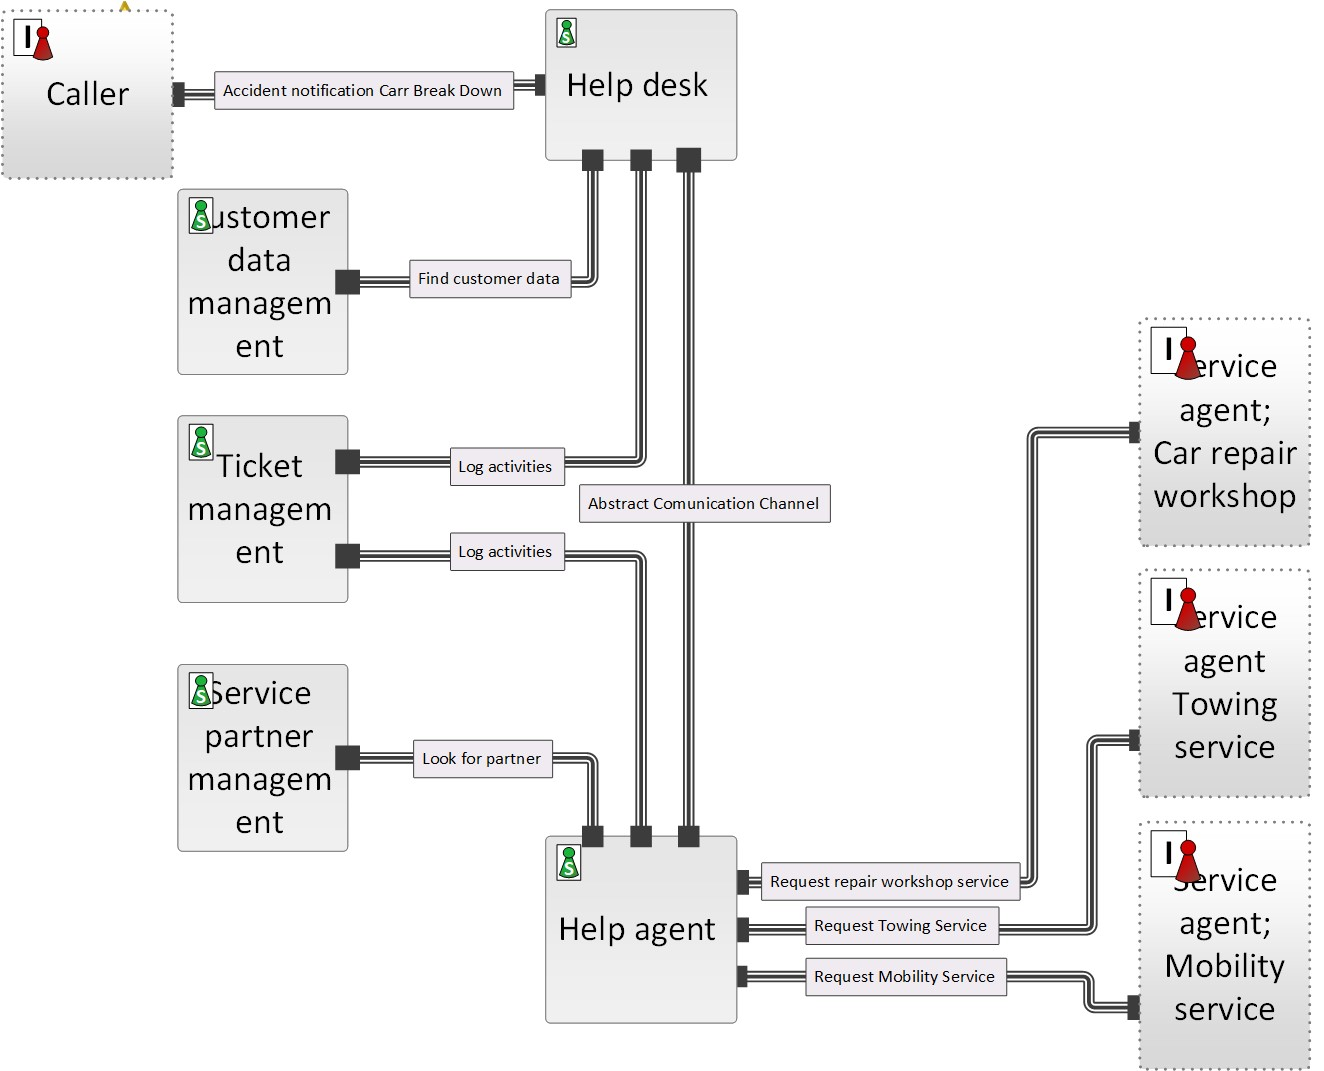
\includegraphics[width=1.0\linewidth]{Figures/Chapter5/figures-hierarchy/Car-Service-Lev6}
	\caption[Subject Interaction Diagram of the Process "Incident Management"]{Subject Interaction Diagram of the Process "Incident Management"}
	\label{fig:car-service-lev6}
\end{figure}

Because we consider the process "Incident management" the border subject "Caller" of the process "Car usage" becomes an interface subject in the SID (details about interface subjects can be found in \cite{Flei12}) of the process “Incident Management”. Figure \ref{fig:car-service-lev8} shows the detailed Subject Interaction Diagram around the subject help desk. \\

\begin{figure}[htbp]
	\centering
	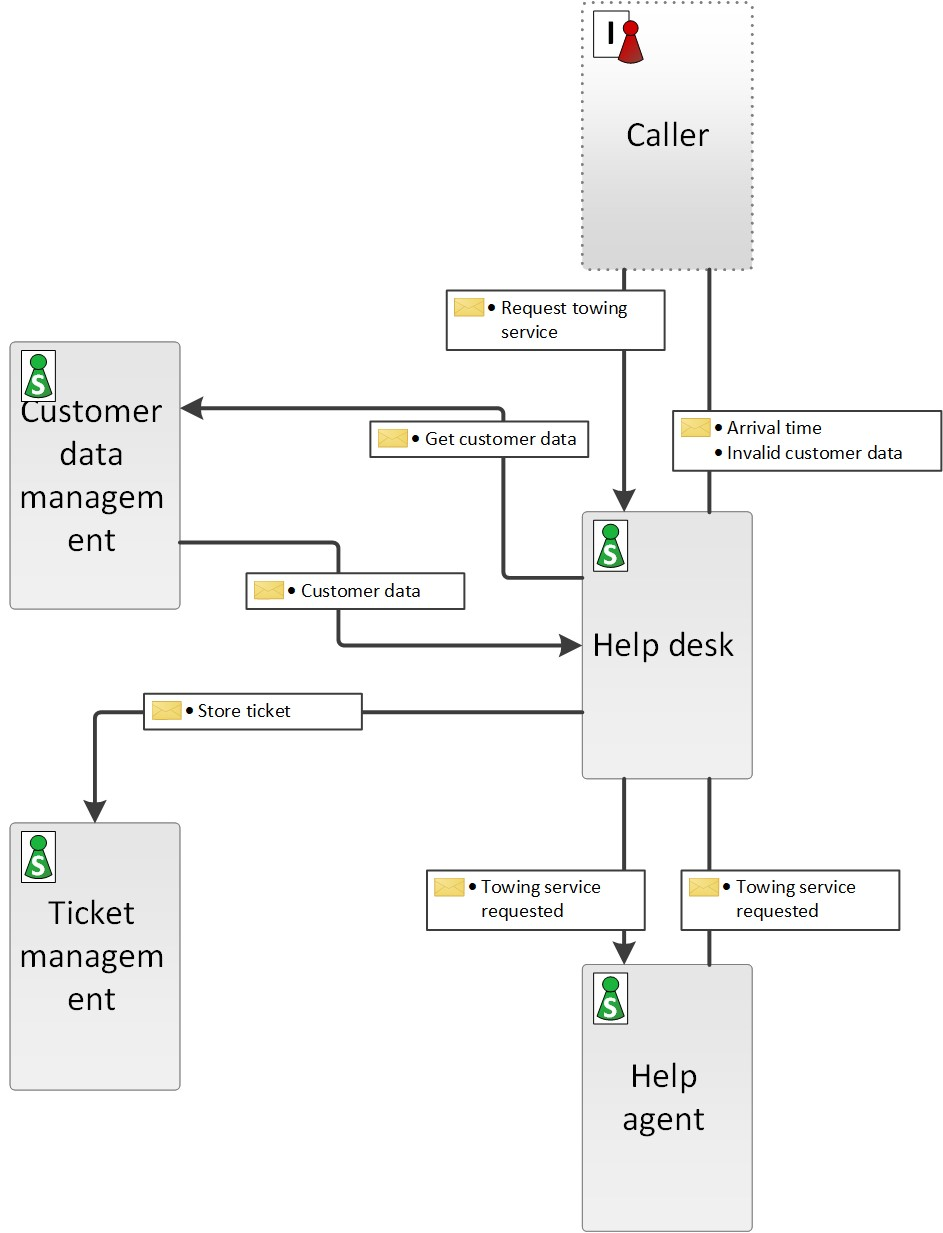
\includegraphics[width=0.9\linewidth]{Figures/Chapter5/figures-hierarchy/Car-Service-Lev8}
	\caption[Subject Interaction around the subject “Help desk”]{Subject Interaction around the subject “Help desk”}
	\label{fig:car-service-lev8}
\end{figure}

Instead of the channels the messages required for a towing service request are shown. A message "Request towing service" comes from the interface subject. This message is accepted by the subject "help desk". The subject help desk checks the customer data received with this message by sending a corresponding the message "Get customer data" to the subject "Customer data management". This subject send the complete customer data back to the subject "Help desk" via the message "Customer data". The subject "Help desk" checks the customer data. If the data are invalid a message "Invalid customer data" is sent to the subject "Caller" and the process is finished.\ 
If the customer data are valid with that data the subject "Help desk" creates a trouble ticket which is sent to the subject "Ticket management". After that the message "Towing service requested" is sent to the help agent which organizes the towing service. The part of the communication structure of the subject "Help agent" in order to organize the towing service is not shown in figure \ref{fig:car-service-lev9}. We only see that subject "Help agent" sends the message "Towing service data" to the subject "Help desk". This message contains all the data about the service e.g. name of the towing company and arrival time. The subject "Help desk" forwards that data to the interface subject "Caller". This behavior is shown in figure \ref{fig:car-service-lev8}.\\



\begin{figure}[htbp]
	\centering
	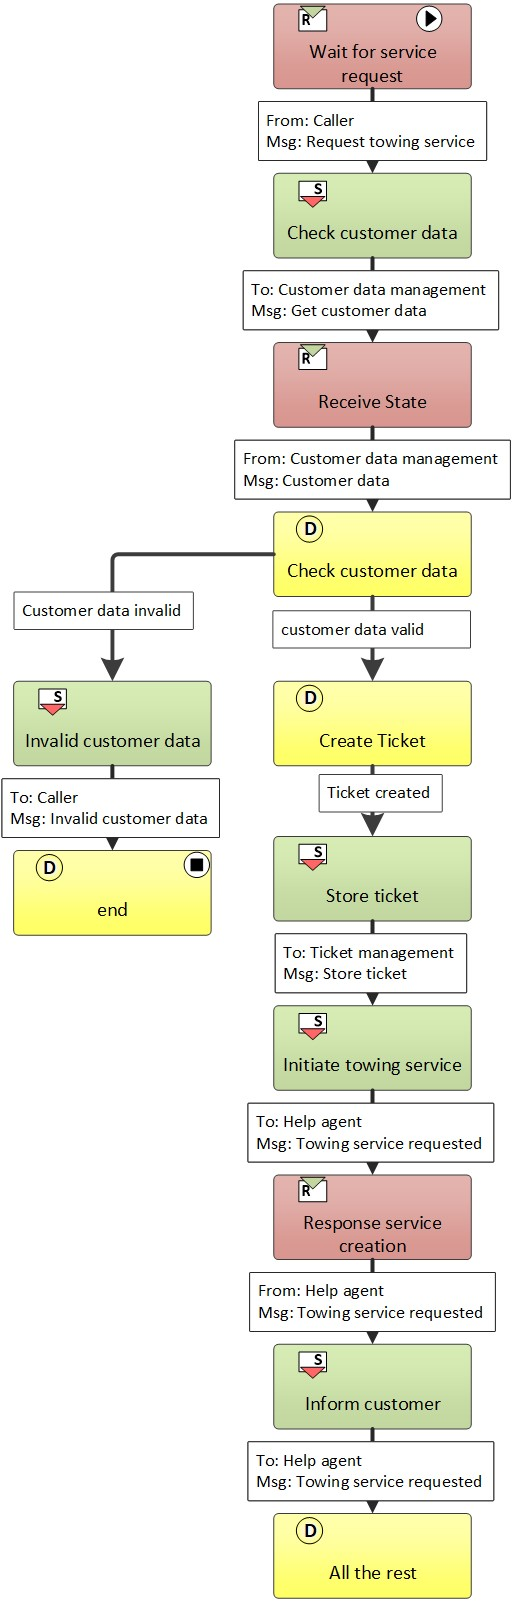
\includegraphics[width=0.7\linewidth]{Figures/Chapter5/figures-hierarchy/Car-Service-Lev9}
	\caption[Part of the Behavior Diagramm of the subject “Help desk”]{Part of the Behavior Diagramm of the subject “Help desk”}
	\label{fig:car-service-lev9}
\end{figure}


The behavior described in the figure above contains the communication with all neighbor subjects of subject "Help desk" including the communication with the interface subject "Caller". From the perspective of this subject the communication of the subject "Help desk" with its other neighbor subjects is not relevant. For the subject "Caller" only the commumication sequence between itself and the subject "Help desk" is relevant. These allowed communication sequences are called the behavioral interface.\\
The behavioral interface between two subjects can be derived from the complete behavior of a subject by deleting the interactions with all the other subjects . Figure \ref{fig:car-service-lev10} shows how the communication sequence relevant for the communication be-tween the subject "Help Desk" and "Caller" is derived from the complete behavior of subject "Help desk".

\begin{figure}[htbp]
	\centering
	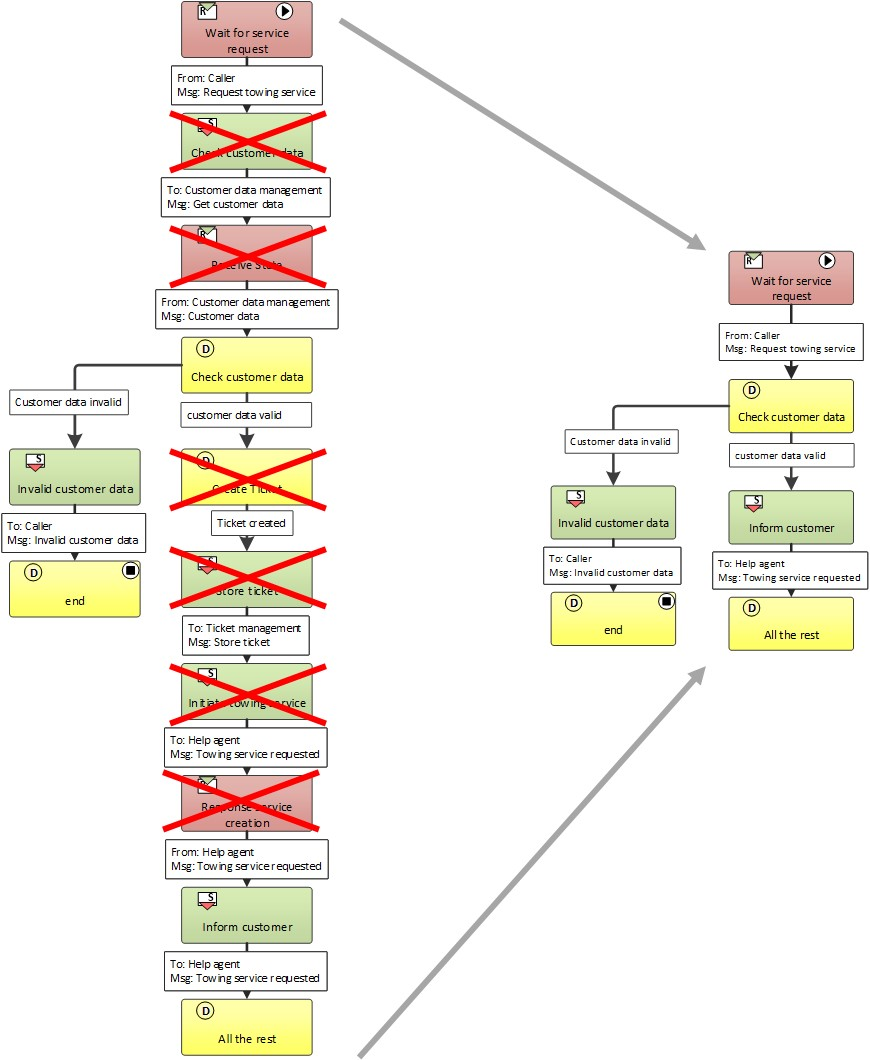
\includegraphics[width=1.0\linewidth]{Figures/Chapter5/figures-hierarchy/Car-Service-Lev10}
	\caption[Deriving the Behavioral Interface from the Subject Behavior]{Deriving the Behavioral Interface from the Subject Behavior}
	\label{fig:car-service-lev10}
\end{figure}

A behavoral interface is always relative to a communication partner. In figure \ref{fig:car-service-lev10} the behavioral interface is relative to the interface subject "Caller". The behavioral interface to the subject "Ticket Management" is different because only the communication activities with this subject are considered.This behavioral interface would be very simple. It consists of only one send activity, sending the message "Store ticket".\\
The behavioral interface relative to a partner subject can be automatically derived from the complete behavior of a subject
(see \cite{article:jCPEX}).


\section{Business Activity Monitoring for S-BPM}\label{sec:BAMinSubjectOrientation}

Monitoring of Business Process looks at running instances. For those it measures metrics, aggregates them to Process Performance Indicators (PPIs) as a business process-related form of Key Performance Indicators (KPIs), reveals deviations (as-is vs. to-be) and report and presents results to people in charge or interested in the value of the PPI. Thus monitoring lays ground for the performance analysis in the key dimensions quality, time and costs of processes and helps identifying weaknesses and opportunities for improvement \cite{book:UntPerform}.
By feeding back information for completed and running instances to analysis monitoring fosters organizational learning, forms an important part of the Business Process Management (BPM) lifecycle \cite{article:SUbjetorientiertBPM} and thus helps implementing the operational level in the closed-loop approach to enterprise performance management \cite{book:processmonitoring} (see figure \ref{fig:Approach-Performance}).
\\


\begin{figure}[htbp]
	\centering
	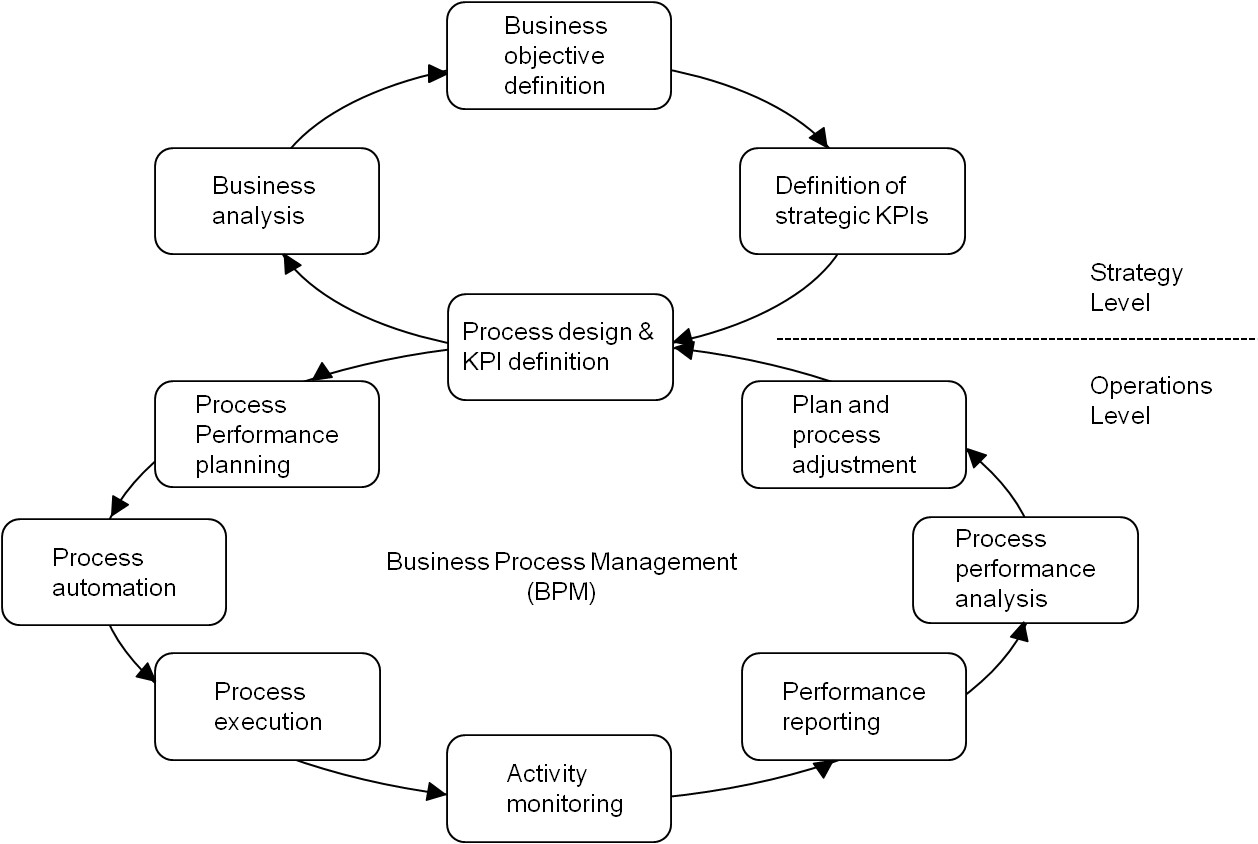
\includegraphics[width=0.8\linewidth]{Figures/Chapter5/Monitoring/Approach-Performance-Mgmt.jpg}
	\caption[Closed-loop Approach to Performance Management]{Closed-loop Approach to Performance Management \cite{book:AnalytInfSys}}
	\label{fig:Approach-Performance}
\end{figure}



\subsection{Architecture }  
A Business Activity Monitoring (BAM) environment supported by Complex Event Processing consists of several elements necessary at build time and at runtime (see figure \ref{fig:BAMArchitecture}) and \cite{book:processmonitoring}, \cite{book:CEPinAction} , \cite{article:BlueprintEventBPM}). At build time a modeling environment should provide tools for designing processes (e.g. Metasonic Build) and defining process performance indicators (PPIs), BAM events, rules, thresholds etc. as well as parameters for their visualization in report and on dashboards. At runtime there are (1) event producers like a process engine (e.g. Metasonic Flow) or an ERP system (e.g. SAP) which feed events into an event cloud or stream (chronologically ordered). (2) Event Processing Agents (EPA) form the event processing logic. They process events based on metrics, event patterns, rules and other parameters specified at design time. Their basic logical functions include filtering and transforming events and detecting patterns among them. Global state elements allow them accessing data from outside the application (e.g. from an ERP system). EPAs put the results of their processing (also to be understood as events) out to Event Consumers (3) like dashboards or process engines. Input and Output Adapters (IA, OA) transform event data between different formats of system elements as necessary. All system elements involved form an Event Processing Network (EPN), in which events are exchanged by communication mechanisms.

\begin{figure}[htbp]
	\centering
	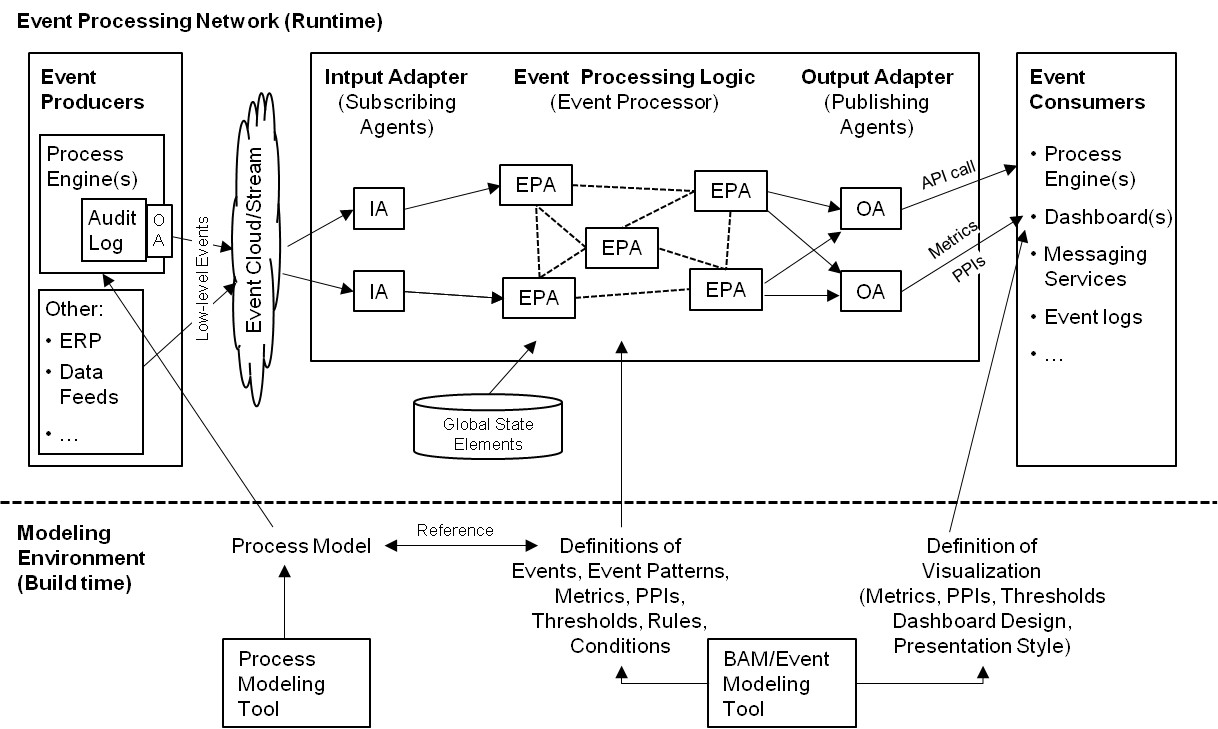
\includegraphics[width=0.9\linewidth]{Figures/Chapter5/Monitoring/Integrated-BAM-CEP-Architecture-27.jpg}
	\caption[Integrated BAM/CEP Architecture 27]{Integrated BAM/CEP Architecture \cite{book:processmonitoring}}
	\label{fig:BAMArchitecture}
\end{figure}



\subsection{Modeling BAM Parameters at Build Time}
As mentioned in the last section it is necessary not only to model the processes, but also numerous pieces of information relevant for a sound process monitoring in the sense of Business Activity Monitoring (BAM model). These can be derived from answers to questions like what, when, how and how often should be measured by whom \cite{book:ProzesseSchmelzer}. The information should also include how single metrics are to be aggregated in order to determine Process Performance Indicators (PPIs). For systematically collecting and documenting the necessary information fact sheets or templates for metrics and performance indicators have been developed \cite{book:KennzahlenIT}, \cite{book:ITControlling}. Figure \ref{tbl:Fact-Sheet}  shows an extract of a sample fact sheet defined for the average processing time of activities (see also \cite{article:SBPMCosting}, \cite{book:MonitoringSubjekt} ).


\begin{table}[htbp]
	\footnotesize
	\centering
	\begin{tabular}[t]{@{}l p{0.5\linewidth} p{0.3\linewidth} @{}}
		\toprule
		\textbf{Attribute} & \textbf{Content}  \\
		\midrule
		 & \textbf{Characteristics}
		\\
		Identifier & Average activity time
		\\
		Description & Average time of a process activity within a certain period
		\\
		To-be value/unit & tbd specifically (min.)
		\\
		Tolerance range/unit & tbd specifically (\%)
		\\
		Escalation Rules/ Actions & In case of violation alert the process owner and start escalation process (tbd specifically)
		\\
		Addressees & Process Owner, Middle Mangement, Accountants (tbd specifically)
		Responsibility	Process Owner (tbd specifically)
		\\
		&  &
		\\
		& \textbf{Measuring and Computing}
		\\
		Measuring Object & All instances of the process 'Purchase Order'
		\\
		(Single) Metrics & Start time and end time of all activities of the process
		\\
		Measuring Method & Read time stamps for beginning and end of activities written by Metasonic Flow 
		\\
		Measuring Frequency & For every single instance as it occurs
		\\
		Algorithms & For computing period: Sum of processing time of all activities divided by number of instances

		\\
		Data Sources (general) & Tables in the database of Metasonic Suite:
		RT\_PROCDESC, RT\_PROCINST, REC\_PARADESC, REC\_RECTRANS, UM\_USER
		\\
		Data Sources (specific) & Activity processing time (for one instance):\newline
		\textbf{SELECT} TIMESTAMP1  \newline
		(\textbf{SELECT} STARTTIME \newline
		\textbf{FROM} RT\_PROCINST \newline
		\textbf{WHERE} RT\_PROCDESC = \textit{process (purchase order)}\newline
		\textbf{AND} ID = \textit{instance (9)}\newline
		\textbf{FROM} REC\_RECTRANS\newline
		\textbf{WHERE} RT\_STDESC = \textit{\textit{state (fill\_in\_form)}}\newline
		\textbf{AND} RT\_PROCINST = \textit{instance (9)}
		Completed instances: see separate fact sheet .
		\\
		Computing Period (time, no. of inst.) & Daily
		\\
		& \textbf{Presentation}
		\\
		Presentation Style & As-is value and to-be value in combination with a spark line showing the historical development, deviation from to-be value in \%
		\\
		Presentation Frequency & Weekly and in case of escalation
		\\
		Archiving & Stored in additional database table, linked with RT\_PROCDESC
		\\
		
\bottomrule
\end{tabular}
\caption{Fact Sheet for a PPI (extract)}
\label{tbl:Fact-Sheet}
\end{table}

Replacing the content column by more formal ontology-based linguistic patterns as suggested by Del-Rio-Ortega et al. (see table \ref{tbl:Fact-Sheet-PPI}) could help relating PPIs to elements of the process model, performing automated analysis \cite{article:ProcessPerfInd} and implementing the measurement at runtime. 

\begin{table}[htbp]
	\footnotesize
	\centering
	\begin{tabular}[t]{@{}l p{0.3\linewidth} p{0.4\linewidth} p{0.5\linewidth} @{}}
		\toprule
		\textbf{Attribute} & \textbf{Linguistic Pattern}  & \textbf{Example}\\
		\midrule
		PPI-<ID> & <PPI descriptive name> & PPI-001 Average time of RFC analysis
		\\
		Process	& <process ID the PPI is related to> & Request for change (RFC)
		\\
		Goals & <strategic or operational goals the PPI is related to> & BG-002: Improve customer satisfaction \newline
		BG-014: Reduce RFC time to response
		\\
		Definition & The PPI is defined as { \newline
			<DurationMeasure> | <CountMeasure> | <ConditionMeasure> |
			<DataMeasure> | <DerivedMeasure> | <AggregatedMeasure> }
		[expressed in <unit of measure>] & The PPI is defined as the average of Duration of Analyse RFC activity
		\\
		Target & The PPI value must { \newline
			be {greater | lower} than [or equal to] <bound> | \newline
			be between <lower bound> and <upper bound> [inclusive] |\newline
			fulfil the following constraint: <target constraint> } & The PPI value must be slower than or equal to 1 working day
		\\
		Scope & The process instances considered for this PPI are {
			the last <n> ones |
			those in the analysis period <AP-x> } & The process instances considered for this PPI are the last 100 ones
		\\
		Source & <source from which the PPI measure can be obtained> &	Event logs of BPMS
		\\
		Responsible & { <role> | <department> | <organization> | <person> } &	Planning and quality manager
		\\
		Informed &{ <role> | <department> | <organization> | <person> } & CIO
		\\
		Comments & <additional comments about the PPI> & Most RFCs are created after 12:00
		\\
\bottomrule
\end{tabular}
\caption{PPI Template based on Linguistic Patterns \cite{article:ProcessPerfInd}}
\label{tbl:Fact-Sheet-PPI}
\end{table}
Friedenstab et al. argue that such linguistic patterns do not fit to the usually graphical modeling of processes which makes integration difficult \cite{article:BPMNActivityMon}. The authors discuss some more approaches to BAM modeling. With regard to the limitations revealed, they present a BAM-related extension of the graphical Business Process Model Notation (BPMN) \cite{article:BPMNActivityMon}.
Using an abstract language syntax based on the Unified Modeling Language (UML) they started defining meta models for language constructs needed for BAM as there are Duration, Frequency, Composed Basic Measure, Aggregated Measure, Filter, Target Definition, Actions, Measure-based Expressions and Dashboard. Figure \ref{fig:Meta-Model} depicts the example for the duration of elements on different levels of detail, where the grey colored parts indicate references to the BPMN specification.

\begin{figure}[htbp]
	\centering
	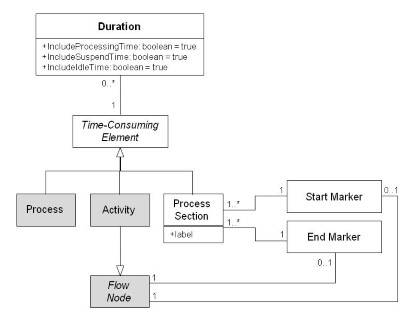
\includegraphics[width=0.9\linewidth]{Figures/Chapter5/Monitoring/Meta-Mode-fo-Duration-relate-to-BPMN-1.jpg}
	\caption[Meta Model for Duration (related to BPMN) 12]{Meta Model for Duration (related to BPMN) \cite{article:BPMNActivityMon}}
	\label{fig:Meta-Model}
\end{figure}


In a second step Friedenstab et al. developed a concrete syntax allowing for modeling the abstract language elements with graphical symbols and text labels. Parts of it are visible in figure \ref{fig:Model-Cycle-Times}. The example shows the BAM model for determining the cycle times of a purchase order process modeled in BPMN (lower part). The upmost part for example expresses the fact that the overall cycle time (Duration) for the last 50 instances (Filter) has to be determined and displayed on the dashboard (Dashboard). Monitoring the average of the overall cycle time for completed instances controls the modeled business logic of the process. If it is above 48 hours goods are delivered with an express shipping if the average cycle time is more than. Otherwise standard shipping is carried out. A deviation also leads to an alert sent to the process owner, while in any case the average is to be presented on the dashboard. The latter is also valid for the third time-related metric in the example, the partial cycle-time for the company-internal part of the process, which is set into relation with the overall cycle time.

\begin{figure}[htbp]
	\centering
	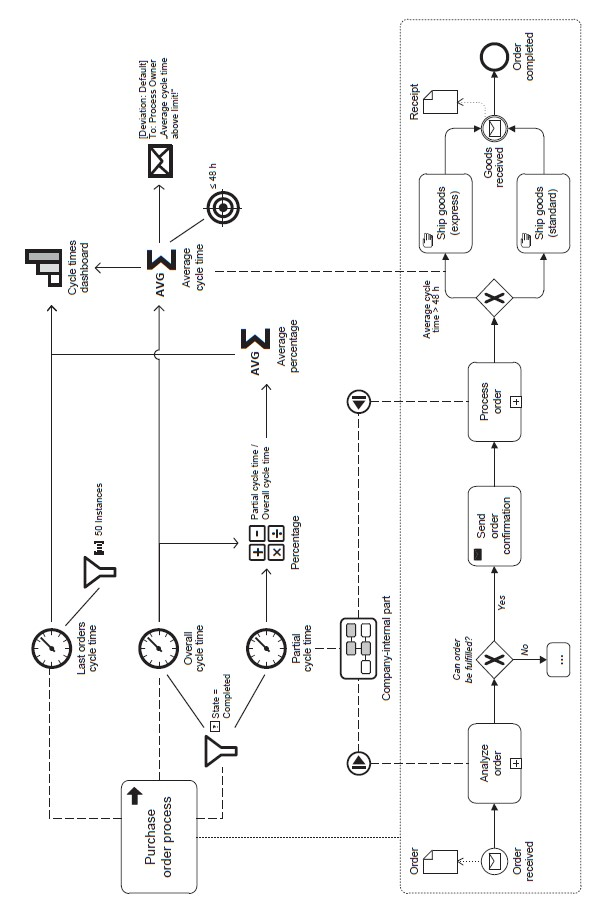
\includegraphics[width=0.9\linewidth]{Figures/Chapter5/Monitoring/BAM Model for Cycle Times.jpg}
	\caption[BAM Model for Cycle Times of a Purchase Order Process based on BPMN 12]{BAM Model for Cycle Times of a Purchase Order Process based on BPMN \cite{article:BPMNActivityMon}}
	\label{fig:Model-Cycle-Times}
\end{figure}


The concept presented by Friedenstab et al. is thoroughly thought-out and clearly and precisely elaborated. The idea now is to adapt it to Subject-oriented Business Process Management and relate the abstract syntax to the S-BPM meta model instead of BPMN. Due to S-BPM being a more precise and comprehensive notation than BPMN \cite{article:BPMNYAWLPatterns} the mapping should be possible without problems. Table \ref{tbl:MonBPMNSBPM} compares the BPMN specification elements used by \cite{article:BPMNActivityMon} with the ones appropriate in S-BPM \cite{Flei12}.


\begin{table}[htbp]
	\footnotesize
	\centering
	\begin{tabular}[t]{@{}l p{0.3\linewidth} p{0.4\linewidth} p{0.5\linewidth} @{}}
	\toprule
	\textbf{BAM Language Syntax Construct} & \textbf{Used BPMN Specification Element}  & \textbf{Suitable S-BPM Specification Element}\\
	\midrule\\
	Duration (Time-Consuming Element) &	Process, Activity, Flow Nodes&	Process, Subject Behaviour States (Function, Send, Receive, Start, End)
	\\
	Frequency
	(Countable Element)&	Process, Activity, Data Objects, Data States &	Process, Subject Behaviour States (Function, Send, Receive), Business Objects and their States 
	\\
	Actions &	Process	 & Process
	\\
	Measure-based Expressions &	Expression, Sequence Flow &	Incoming Message
	\\
	\bottomrule
\end{tabular}
\caption{BPMN and S-BPM Specifications used in BAM Constructs}
\label{tbl:MonBPMNSBPM}
\end{table}

The remaining constructs as well as the extensions do not depend on the process modeling language and thus are not included in the table.
On the other hand S-BPM, following its paradigm of regarding subjects, predicates and objects as equally important parts of a process, offers the subject as an additional specification element to add . In figure \ref{fig:Meta-Model-S_BPM} we modified the picture of figure \ref{fig:Meta-Model} by replacing the BPMN by S-BPM elements and adding the subject. This allows modeling the determination of the overall time a subject (respectively the allocated resource(s)) spends on working on a process instance. This is of interest for cost-related analysis.

\begin{figure}[htbp]
	\centering
	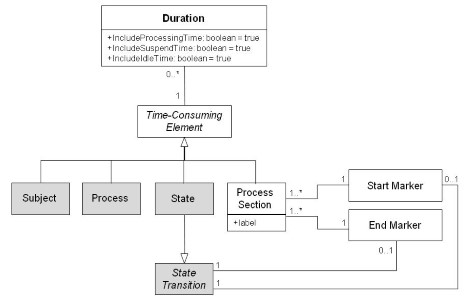
\includegraphics[width=0.9\linewidth]{Figures/Chapter5/Monitoring/Meta-Mode-fo-Duration-relate- to-SBPM.jpg}
	\caption[Meta Model for Duration (related to S-BPM)]{Meta Model for Duration (related to S-BPM)}
	\label{fig:Meta-Model-S_BPM}
\end{figure}


In order to show how the BAM language syntax constructs can be related to subject-oriented models we designed the purchase order process in S-BPM. Due to missing information in the BPM model some assumptions were necessary like who performs the process steps (subjects). We then added the BAM modeling symbols to create a monitoring model similar to that in figure \ref{fig:Meta-Model-S_BPM}.
The result is depicted in the following graph. In the lower part it includes the subject interaction diagram (SID) of the process. The SID shows the subjects involved and how they coordinate themselves in the course of action by exchanging messages. In the monitoring model in the upper part a difference can be seen. The partial cycle time for the company-internal activities can be modeled by just relating the clock symbol to the subject "Sales". In the example this subject represents all steps carried out within the organization. In the same way we can determine the cycle time for the other subjects.

\begin{figure}[htbp]
	\centering
	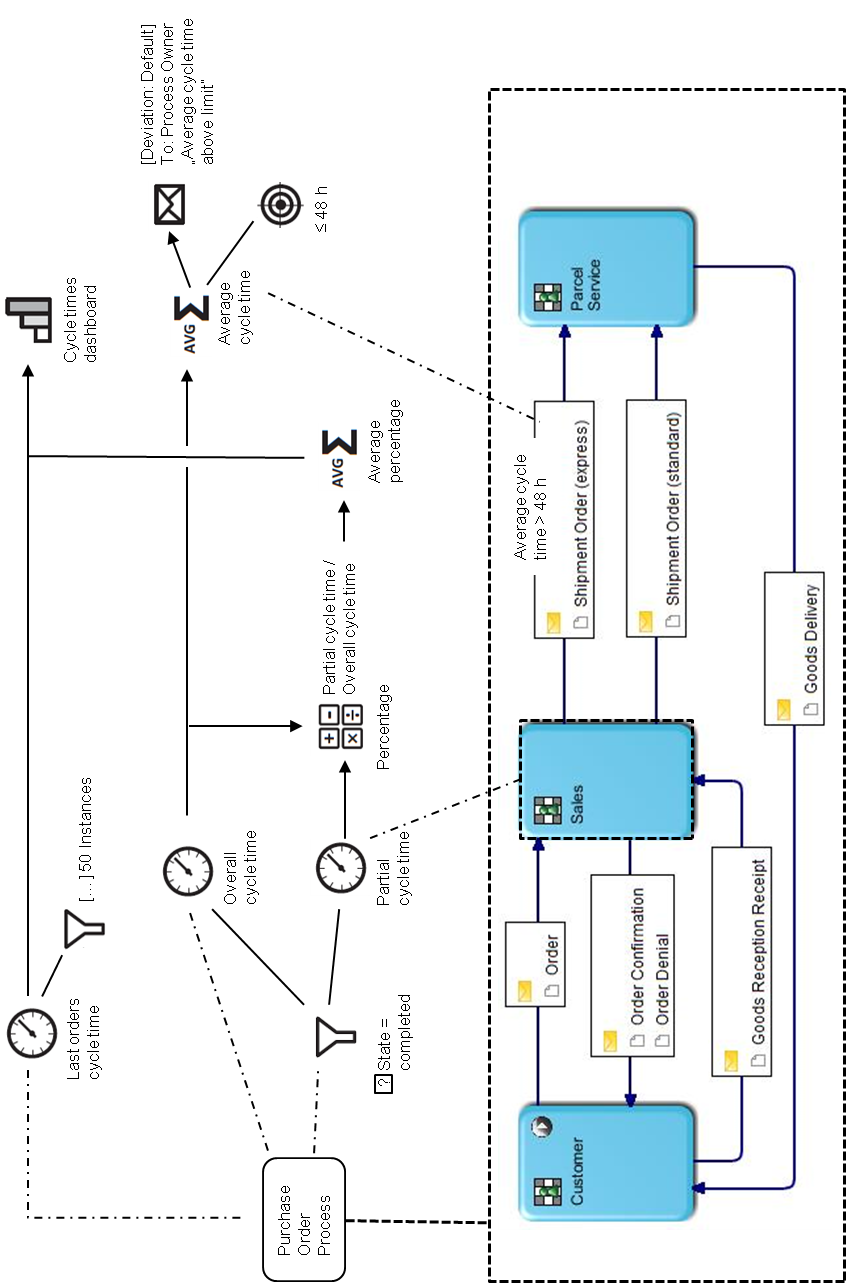
\includegraphics[width=0.9\linewidth]{Figures/Chapter5/Monitoring/BAM-Model-fo- Cycle-Times-of-a-Purchase-Order-Process-based-on-S-BPM.png}
	\caption[BAM Model for Cycle Times of a Purchase Order Process based on S-BPM]{BAM Model for Cycle Times of a Purchase Order Process based on S-BPM}
	\label{fig:Cycle-Time-SBPM}
\end{figure}

Given a special information demand a more granular modeling of BAM parameters is possible on the subject behavior level. Figure \ref{fig:BAM-Cycle-Time} for example details the behavior of "Sales" including all receive, send and functional states walked through by the subject. The symbols indicate that the average cycle time between order reception and confirming the order to the customer should be measured. In the same way cycle times between states in behaviours of different subjects can be modelled.


\begin{figure}[htbp]
	\centering
	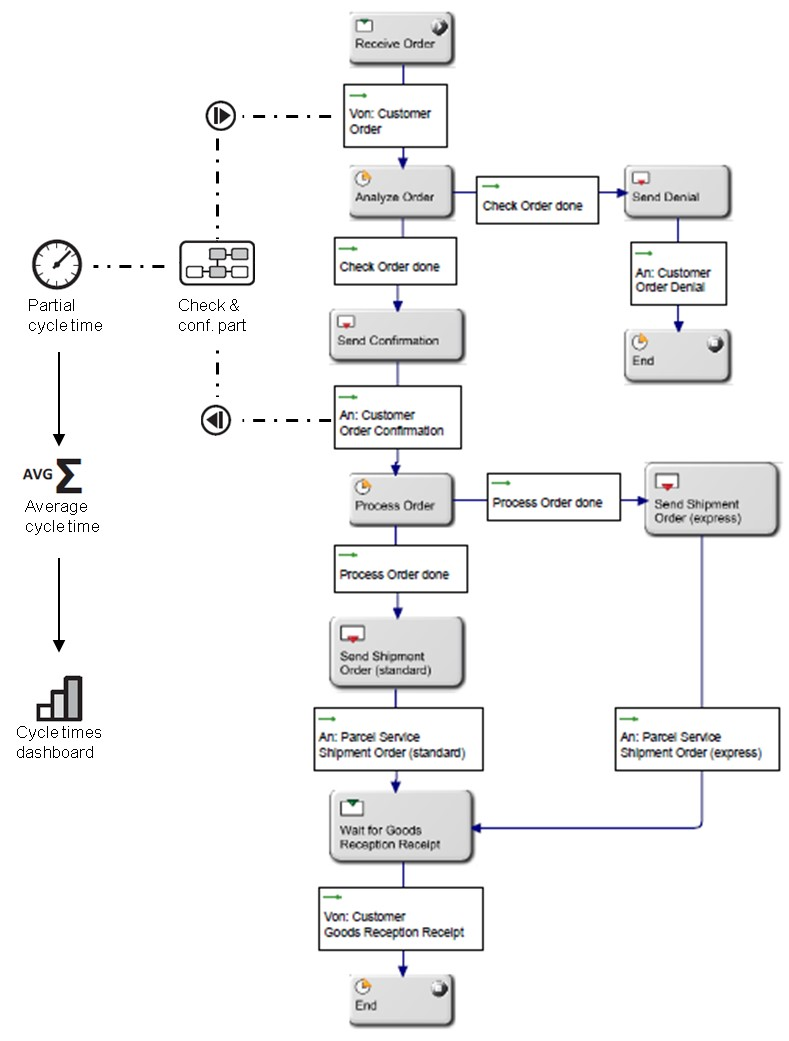
\includegraphics[width=0.9\linewidth]{Figures/Chapter5/Monitoring/BAM-Model-for-Cycle-Time-of-a-Process-Section-based-on-S-BPM.jpg}
	\caption[BAM Model for Cycle Time of a Process Section based on S-BPM]{BAM Model for Cycle Time of a Process Section based on S-BPM}
	\label{fig:BAM-Cycle-Time}
\end{figure}

Back on the level of subject interaction diagram we could also model to determine the overall time for receiving (waiting), sending and doing, both by process and by subject. Modeling on the two diagram levels reduces complexity.

\subsection {Conclusion and future Work}
This contribution systematized Business Process Monitoring and shed some light on the current state of monitoring in the context of S-BPM. Starting there we emphasized Business Activity Monitoring and took a closer look to the modelling of BAM parameters. We showed that the approach for BPMN presented by Friedenstab et al. can be adapted to S-BPM with little effort and that S-BPM shows additional potential to further develop the concept.
This is where future work needs to continue. The first step to go should be elaborating, detailing and tailoring the modeling language for the needs of S-BPM in order define a comprehensive basis for the succeeding task of developing easy-to-use software tool support. 
\\
The BAM modeling tool should make use of the model data created by the process modeling tool and add its results to a combined model base both for process execution and BAM. The third step would then be to build BAM functionality which at runtime processes events according to the subject-oriented BAM models. There is some evidence that S-BPM provides good premises to support event processing \cite{article:nondeterministicEvents}, e.g. by integration of a CEP Engine or single Event Processing Agents as subjects into processes. This has to be proven by a thorough investigation of the interrelationship and integration potential of CEP and S-BPM concepts and solutions. Generating code for BAM functionality out of the BAM model is another challenge to tackle \cite{article:BPMNActivityMon}. With the clear formal semantic of its underlying process algebra the S-BPM modeling language allows this for process models \cite{Flei12}. Consequently it seems to be worthwhile to investigate the possibilities of code generation out of BAM models too. 
\\
\\

\section{Subject Oriented Project Management}

Subject orientation is focused on networks of indeppendent systems, which coordinate their cooperation by exchanging messages. The involved system may belong to different organisations.
In our global economy enterprises cooperate around the globe in order to create services or manufacture products for customers which are also distributed all over the world. The challenge of the cooperating partners as a federation of independent systems (virtual enterprise, VE) is to establish smooth cross-enterprise communication to reach the common objectives \cite{article:VirtualEnterprise}. Information and communication technologies (ICT) are essential to create a federation of independent software systems suitable to execute business processes across the involved companies. 
\\
Figure \ref{fig:DogFoodShop} shows an example of an order-to-cash scenario where federated applications support a cross-company business process. A dog food store sells its products via internet. It commissions a transportation service provider to deliver the ordered products to the customer, who confirms the reception of the goods. The store deducts the money from the customer's bank account. The process steps are facilitated by several independent software applications and message exchanges (order, order confirmation, delivery notification etc.) enabled by respective communication systems.


\begin{figure}[htbp]
	\centering
	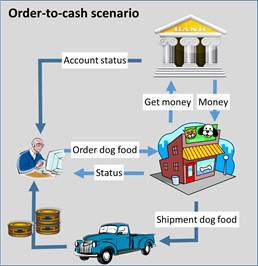
\includegraphics[width=0.6\linewidth] {Figures/Chapter5/Project/DogFoodShop.jpg}
	\caption[Order-to-cash scenario in a federation of enterprises and applications (simplified)]{Order-to-cash scenario in a federation of enterprises and applications (simplified)}
	\label{fig:DogFoodShop}
\end{figure}

Developing such a mutually adjusted solution by a federation of independent enterprises requires a project management approach different from traditional software development projects taking a process perspective (cf. \cite{book:ProjectHistory}). Therefore our focus is on how to implement loosely coupled systems for exchanging information between independent partners, rather than tightly coupled solutions for sharing information or other resources.
The section is structured as follows. First software development methodology and its elements are reviewed with respect to developing federated systems. This leads to our proposal of a software development approach for federated systems based on subject orientation. 
\\
\subsection{Background}

\subsubsection{\textbf{Recommendations for creating federated systems}}
When independent enterprises develop a federated system a lot of managerial and technological aspects have to be considered, particularly with respect to managing collaborative business processes. This is reflected in the following recommendations (cf. \cite{book:PMThirdWave} , \cite{ChallengesDistPM} ):
\begin{enumerate}
	\item Start the foundation of a federation and identify members.
	\item Identify and describe the business services that organizations can provide or they need from partners in service level agreements.
	\item Harmonize the enactment of collaboration by coordinating the participating organizations according to defined business processes and identify the systems required for the federation.
	\item Integrate the identified and implemented services/systems into the intended application. 
	\item Maximize the autonomy of organizations when collaborating, thereby ensuring organizations to benefit most from their own business objectives.
	\item Represent the partnerships between collaborating organizations when collaborating, and update changes in partnership.
	\item Guarantee the business privacy of organizations in the course of collaboration.
	\item Allow partners and other third parties to monitor, measure, and oversee the execution of business processes.
\end{enumerate}


\subsubsection{\textbf{Federation of enterprise information systems}}
\cite{article:VirtualEnterprise} define virtual enterprises and federations of enterprise information systems as follows: "\textit{The Enterprise partners' Virtual Enterprise (EP VE) is the federation of partners in the community that come together to achieve the goal of a federated distributed system environment, sharing their resources, and collaborating to achieve a common goal: the Federated System VE (FS VE). The partners in the federation retain autonomy over their resources, deciding which resources (personnel, resource dollars, equipment, etc.) are sharable for achieving this goal. The results of this VE are then useable by the partners in furthering their individual systems. The FS VE is seen to be a virtual system of distributed processing components (hardware and software), which are physically implemented and managed by the partners. It is a federation of the partners' systems, where each system retains its autonomy over all processing system components and sharable data/information. Retaining autonomy means defining which data or information and software/hardware assets will participate in the federation and be accessible and usable by other systems in the federation.}"\\
The definition shows that the focus is on sharable resources. This means when setting up a federation the VE members need to clarify ownership of the shared resources as well as access rights and the rights to change those. Such an approach often implies tight coupling of the involved enterprises and the related resources. Entities leaving a federation then cause difficulties with respect to separating involved systems (changing access rights) and sorting out ownership of information.
Alternatively, information can be exchanged between the partners by messages, implying only a loose coupling of the involved systems. In this case the partners only need to agree upon structure and meaning of the data, e.g., using XML schemes, and upon the implementation of the message exchange, e.g., by web services. 
\\
\subsubsection{\textbf{Software development methodology}}
\textit{"A software development methodology is a collection of procedures, techniques, tools and documentation aids which help developers to implement software systems"}  \cite{book:ISDevelopment}. It may include modeling concepts, tools for model-driven architecture, integrated development environments (IDEs) etc. The so-called magic triangle (see figure \ref{fig:Triangle}) summarizes the various aspects of a software development methodology \cite{book:SoftEng}.

\begin{figure}[htbp]
	\centering
	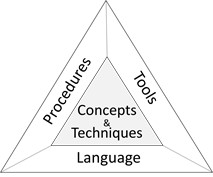
\includegraphics[width=0.6\linewidth] {Figures/Chapter5/Project/Triangle.jpg}
	\caption[Magic triangle of software development methodologies]{Magic triangle of software development methodologies}
	\label{fig:Triangle}
\end{figure}

Concepts and Techniques are used to create models of the software to be implemented, and are thus significantly influencing which languages, procedures and tools are utilized. The applied concept implies the artifacts to be produced, of which the executable software system is the most important one. The Language is used to create the artifacts and tools. Procedures describe the sequence in which the activities for creating the various artifacts are executed. While languages and tools can be replaced without impacting concepts and procedures, the latter are decisively determining the shape of a software development environment.
\\
\subsubsection{\textbf{Modeling concepts}}
Developing a federated system like the dog food store requires modeling cross-company business processes and the entities performing activities in these processes.
\paragraph{Business process modeling} 
There are various approaches for specifying business process models. IT implementations of those models are called process-controlled applications [7] or workflows. The modeling approaches can be distinguished in three classes: (i) Control flow-based specifications put the focus on the activities. (ii) Object-based models mainly describe business objects and the sequence of operations to manipulate them. (iii) Communication-based models focus on the active entities in a process which exchange messages in order to coordinate their work.
By their nature the latter are promising candidates for modeling federations of systems. Business Process Model and Notation (BPMN), the currently most widely discussed modeling language, contains elements for the description of control flows and communication in business processes. In the following we discuss its communication-oriented features.
To model communication BPMN provides so-called pools, each representing a process that can exchange messages with processes in other pools. Conversation diagrams are the means to describe this mechanism: However, they do not allow specifying the sequence in which messages are exchanged. Although the sequence can be captured by collaboration diagrams, the semantics of sending and receiving messages is not precisely defined. For instance, it remains unclear whether messages are exchanged synchronously or asynchronously. Additionally a certain message from a pool can only be received in a single activity state, but not in other states. Choreography diagrams in BPMN also define the allowed message sequence between pools. [8] describe a choreography-based tool for specifying global processes. The problem is that choreography specifications cannot contain data. As a consequence a modeler can only describe message sequences being covered by regular expressions, which is the lowest level in the Chomsky hierarchy. This fact makes it impossible to model a behavior like the following: Pool S sends n messages of a type X to pool R. After that S sends a message Y to R. Subsequently S expects m messages of type A from pool R, which received the n messages of type X. The reason for that is that the messages cannot be counted, because data are not allowed in BPMN choreographies.
Given these properties of BPMN this notation has significant draw backs for modeling communication, hindering the precise development of federations of systems.

\paragraph{Multi-agent systems modeling}
The term agent has multiple meanings. We follow the definition given in [9]: An agent is an entity that performs a specific activity in an environment of which it is aware and that can respond to changes. A multi-agent system (MAS) is a system where several, perhaps all, of the connected entities are agents. The most important property of agents is their controlled autonomy: They independently execute their role-specific behavior, and in multi-agent systems they communicate with each other. These properties are alike those of federated systems which therefore can be considered as multi-agent systems. This means that software development methodologies for agent-oriented software (for an overview see [8]) can help developing federations of applications.
\\
\subsubsection{\textbf{Procedures}}
Software Life Cycles (SLC) build a framework for software development procedures. All software development projects follow a series of phases. While software life cycles can be defined in many different ways, each of them comprises the following generic activities:
\begin{list}{-}{spacing}
	\item Project conception or initiation
	\item Planning
	\item Execution with specification and implementation activities
	\item Termination
\end{list}

In the traditional waterfall approach these activities are performed in the sequence shown above. Other life cycle concepts propose overlapping the development steps, suggest alternatives like the V model or agile development procedures like Extreme Programming and Scrum. \cite{article:ObjectOrientedSWdev}, \cite{book:SoftEng} and \cite{book:ISDevelopment} give an overview of the various approaches.
\\
\subsubsection{\textbf{Work break down structure (WBS)}}
The work break-down structure describes the artifacts to be created in a project in a hierarchical way. A work break-down structure element may be a product, data, service, or any activity results contained in the software life cycle or any combination thereof. A WBS also provides the necessary framework for detailed cost estimating and control along with guidance for schedule development and control. The top level of the WBS should identify the major phases and milestones of the project in a summative fashion. Consequently, the phases used in the top level depend on the software development methodology applied in a project. The first level can either represent the phases used in the software life cycle or the major artifacts of the system to be developed. In case the top level is SLC-oriented it might be built by requirement specification, software architecture, programming, test etc. In the case of an evolutionary life cycle there will be topics like Release 1, Release 2 etc., followed by headlines like requirement specification on the second level.
Another alternative is to use top level headlines corresponding to artifacts created by modeling activities, such as 'create communication structure' or 'describe subject behavior'. 
\\
The WBS is created during the planning phase of a project life cycle. During this phase the project manager works with the project team to make sure that the client's needs are addressed and the project is planned completely and approved by the client prior to any sort of production beginning on the project.

\subsubsection{Organisational break down structure and software architecture}
An organizational breakdown structure (OBS) complements the WBS and resource breakdown structure of a project. Project organizations can be broken down in much the same way as the work or product. The OBS is created to reflect the strategy for managing the various aspects of the project and shows the hierarchical breakdown of the management structure. Hence, the work break down structure has a significant impact on the organizational structure of the project team. The same holds for the phases of the software life cycle and the system architecture influencing the work break down structure. Conway’s law states “organizations which design systems ... are constrained to produce designs which are copies of the communication structures of these organizations” \cite{article:ConwaysLaw}. A variation of Conway’s law can be found in [12]. "If the parts of an organization (e.g., teams, departments, or subdivisions) do not closely reflect the essential parts of the product, or if the relationship between organizations do not reflect the relationships between product parts, then the project will be in trouble... Therefore: Make sure the organization is compatible with the product architecture” \cite{book:OrgPatternsAgile}.
As we look at developing federations of systems with a federation of independent project teams, the system architecture needs to be aligned with the multiple project team structure.
\\

\subsection{Software Development Methodology For Federated Systems}
The software development methodology for federated systems proposed here is based on Subject-oriented Business Process Management (S-BPM)  


\subsubsection{Development as a multiple-team structure}
We now assume that the dog food order-to-cash scenario does not yet exist. The store wants to extend its services for the customers by offering online shopping and home delivery. In order to reach this business objective it takes the initiative to found a federation of enterprises which combine their services and develop a corresponding federation of systems.
Each federated enterprise establishes a project team, working on their parts of the solution independent from each other. This leads to a multiple-team project on the federation level \cite{book:OrgPatternsAgile}. As the teams belong to different, independent companies they all have their own development culture and methodology.
Since there is no single line management who can assign an overall project manager, the federation members need to agree on a project leader and the competencies related to this role. As the initiator of a federation has the most interest in the development of the federated solution it might be helpful that this company, in our case the store, recruits the leader.

His or her major task is to ensure smooth communication between the independent teams, respectively their managers. The project teams needs to coordinate how the systems they are developing communicate with each other. Their major communication paths are predefined by the communication structure of the system federation. This strategy leads to a high socio-technical-congruence. Figure \ref{Multiple-team} (CS: no missing) shows the team and communication structure of the dog food order-to-cash federation.

\begin{figure}[htbp]
	\centering
	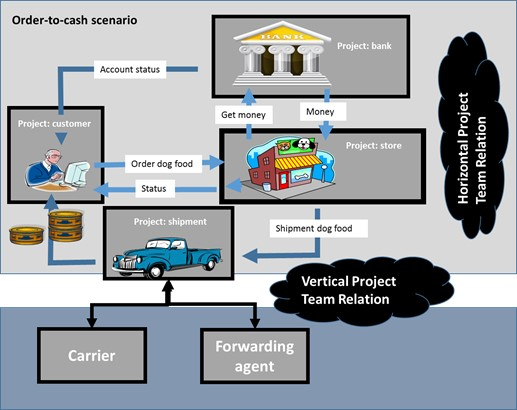
\includegraphics[width=0.6\linewidth] {Figures/Chapter5/Project/MultipleTeam.jpg}
	\caption[Multiple-team project and its communication structure]{Multiple-team project and its communication structure}
	\label{fig:Multiple-team}
\end{figure}

Beside that top-level communication implied by the problem structure, each team can use services offered by other enterprises. Figure 6 reveals that the shipment company uses the service of carriers and forwarding agents, in order to implement the transportation service offered to the dog food shop. This communication relation is of no interest for other federation members and thus should not be visible to the top level teams. It belongs to the internal issues of the shipment project team.
\\
\subsubsection{Development process for federated systems}
 The artifacts to be created according to subject orientation need to be developed by a federation of teams related to the subject interaction structure.
 
\paragraph{Specification of the communication structure}\
The communication between the various members of the federation needs to be specified in more detail. This is done by assigning a subject to each member of the federation and defining the messages exchanged between the subjects. Together with the data transported by the messages a communication model of the system federation is defined. The advantage of the subject-oriented approach is that the system communication structure is directly in line with the communication structure of the corresponding developing teams. The result of that step is the subject interaction diagram (SID). 

\paragraph{Specification of the subject behaviour}\
After defining the communication structure the behavior of each subject is specified. The modelers describe the allowed sequence of messages exchanged on top level and the internal functions of the individual systems. These internal functions represent the services executed by the corresponding federation partner either directly or supported by other service providers. They also encapsulate the communication with those sub-contractors as it is of no interest on the top level of the federation.\\
The behavior of a subject is mainly defined by the corresponding project team, however, in close coordination with the teams responsible for the partner subjects. The teams only need to make sure a message sent to a partner has a receive state in the corresponding subject behavior and vice versa. This pairwise coupling means, e.g., that the behavior description of the shipment company has to contain a state for receiving the “Transfer order” message, transmitted by the related send state in the behavior diagram of the dog food store subject. In order to correctly model these interactions the responsible project teams need also to agree on the interaction sequence of the subjects. However, their internal task behavior (i.e. sequence of functions for task accomplishment) might not become visible to others, as is specified decentralized and might not be shared at all. 

\paragraph{Implementation of the input pool}\
The input pool is the abstract concept for defining the semantics of message exchange. Partners exchanging messages need to agree on how they implement the input pool semantics. Sending requires the sending subject to execute a function to deposit a message in the input pool of the receiver. For each subject doing so an implementation agreement is necessary. Since an input pool is owned by exactly one subject, the functionality for accessing it is local and does not need to be coordinated with the partners. In most cases input pools are implemented as web services.

\paragraph{Implementation of subject behaviour}\
Each team has to implement the behavior of its subject. This means they have to ensure that depositing and removing messages (including business objects) in or from the input pool are executed and internal functions are invoked in the specified sequence. Workflow engines are appropriate tools for implementing that functionality.\

\paragraph{Implementation of internal functions}\
The internal functions realize the kernel of the service contributed by a partner to a federated application. Messages are the means to cause the invocation of an internal function, and they transport its result to a partner subject. Internal functions can be based on existing systems, e.g., an SAP client.  They also can be implemented using another federated solution, or being developed from scratch. The way an internal function is realized is a local decision taken by the corresponding project team.

\paragraph{Operation of a federated system}\
Beside the development and deployment the non-functional aspects of a federated system need to be agreed upon by the contributing partners. For this purpose they negotiate service level agreements (SLA) defining response time, down time, reaction time in error cases etc. The SLA also includes business aspects like costs and regulations for exceptional situations like a member leaving the federation and bringing in another one.

\subsubsection{\textbf{Federated work break down structure}}
The various activities described so far can be organized in a federated work break-down structure as shown in figure \ref{fig:WBSDog}.

\begin{figure}[htbp]
	\centering
	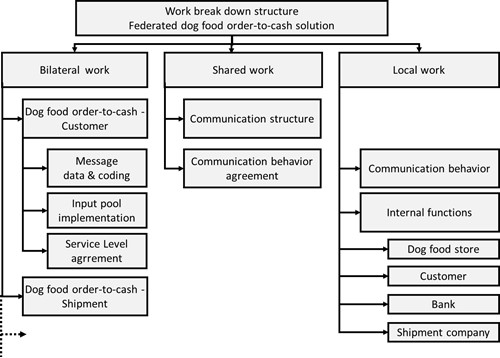
\includegraphics[width=0.6\linewidth] {Figures/Chapter5/Project/WBSDog.jpg}
	\caption[Work break down structure for the development of a federated system]{Work break down structure for the development of a federated system}
	\label{fig:WBSDog}
\end{figure}

The tasks can be divided into three types:\\
\textbf{Joint work} concerns the top level of the federation and therefore is done collaboratively by all members of a federation. The major issue on this level is to agree on communication structure and behavior of the entire system, while the behavior of each subject can be described individually by the corresponding member of the federation.\\
\textbf{Some work can be done bilateral}. Communicating partners, e.g., agree on the coding of the business objects and the implementation of the input pool. They also define the service level agreements.\\
\textbf{Local work} comprises activities of the development teams which do need to be coordinated with teams of other federation members. A major example in this context is the set of internal functions of each subject, being a local matter, and developed following the particular culture and methodology of the respective team.
\\


\subsection{Conclusion and Further Work}
We have presented an approach for developing federated systems. The concept considers the characteristics of virtual enterprises combining the services of the partners to satisfy customer needs while keeping legal, organizational, technological and cultural independence.
Our communication-oriented view follows the idea that the decentralized structure of federated systems needs to be reflected in the organizational structure of multiple project teams for developing such systems. Those teams belong to separate enterprises and are mutually independent with respect to methodology, technology etc. they use to develop their individual part of the federated system. 
The proposed approach establishes a layer above the enterprise-specific environments. It helps building coherence on the top level of the federated system solution, while the teams, system elements etc. on the individual level of each federation member keep the highest degree of independence.
\\

\section{Subject-Oriented Fog Computing}

Many scenarios related to digitalization increasingly (i) require an easy-to-customize development environment, (ii) capture on-the-edge systems or devices under the control of users or responsible stakeholders. Typical examples are home support systems in healthcare, maker environments producing local goods, and intelligent transport control systems for smart regions. Developing such applications requires architectures that allow to network or compose systems in a modular, while effective and efficient way \cite{article:SurveyCompConcepts}. During the last years, with the advent of advanced equipment and technologies, such as production devices for the private consumer market, networked applications have become common. As a consequence of this trend, a significant issue also appears, namely the increases in the demand of both communication and execution capability. New applications, such as home care support systems, all deal with complex interaction operations, which should be understood by users, and thus require a high level of abstraction \cite{article:FogHealthcare},\cite{article:MobilecloudComp}. 
\\
Such demands pose significant challenges to existing development paradigms, particularly in terms of edge computing and stakeholder-oriented communication capacities (cf. \cite{article:SurveyCompConcepts},\cite{article:FogHealthcare}]). Using behavior abstractions aligning stakeholder needs with communication and processing capabilities in this context is an appealing idea. For instance, in-situ care support devices can be utilized to handle the tasks of preparing the pharmacy order or they can be employed to collaborate with each other to transmitting maintenance messages and sharing resources \cite{article:FogHealthcare}. Besides network technologies, mobile cloud computing is a typical enabler for this demand \cite{article:MobilecloudComp}.\\ 
However, according to Syed et al. \cite{article:FogPattern} purely cloud-based systems typically require low latency, support for heterogeneity, mobility, geographical distribution, location awareness, etc. Consequently, Fog Computing (FC) as a near-the-edge-computing paradigm has been defined as a collection of various small distributed clouds deployed closer to the systems or devices at the edge of a communication network (ibid.). Fog applications can be structured along several dimensions, either directly or indirectly referring to stakeholder interaction \cite{article:OoTAnalytics}:
\begin{list}{-}{spacing}
	\item Geo-distribution: wide (across region) and dense - high population of events, such as ramp accesses in traffic, sensor systems in production halls, clustering medical devices in home healthcare application development
	\item Low/predictable latency: tight within the scope of a certain location - intersection, production isle, treatment room
	\item Fog-cloud interplay: data at different time scales - sensors at intersection/traffic info at diverse collection points, supply chain monitoring/production control in process industry, monitoring body condition/treatment planning procedure in healthcare
	\item Multi-agencies orchestration: Agencies that run the system coordinate policy implementation at the same time, e.g., traffic authority runs light system while controlling law policies in real time; active elements for production control implement also governance regulations; home healthcare support is effective with respect to medical treatment and personal well-being.
	\item Consistency: adjusting demands and capabilities, such as getting the traffic landscape demands a degree of consistency between collection points, aligning engineering with production processes, or ensuring well-being while adapting medication to patient needs.
\end{list}

In this contribution, we present Subject-oriented Fog Computing (SFC), a choreographic approach and multi-layered infrastructure for Fog Computing. Separating modeling from organizational and technical implementation along a staged procedure it aims for supporting system architects, designers, and developers, who are interested in stakeholder interactions when building Fog Computing solutions. We propose a development and software architecture scheme without platform dependencies, open for various networked settings. It is based on behavior abstractions termed subjects that integrate a socio-technical design perspective, and allows composing applications from a stakeholder perspective (cf. [6-8]).
In the following section we review related research to developing fog applications according to stakeholder needs in various domains. Subsequently, we introduce SFC based on a System-of-Systems perspective, and provides an exemplary case from developing home healthcare support systems. Finally, we conclude summarizing SFC and indicating further standardization activities. 

\subsection{Fog Computing and Subjects}

We introduce Fog actors by starting with the encoded System-of-System perspective, sketching the federated nature of choreographic ecosystems (subsection above). We then provide the basic modeling notation and exemplify Fog actors as subjects for a home healthcare scenario. Finally, the corresponding Fog runtime system is sketched in terms of its application along the organizational and technical development phases. 

\subsubsection{Federated Systems}
When considering Fog Computing as an addition to cloud ecosystems we expand software architectures to include systems outside the software system which interact with the software system \cite{article:FogPattern}. Each component of the ecosystem can be represented as a system using behavior models. Thereby, cloud ecosystems can serve as service providers for the nodes of the network (of applications). The Fog network enriches the cloud ecosystem, e.g., for specific purpose like home healthcare with domain-specific models.\

Since these enrichments are compound systems, a System-of-Systems (SoS) perspective helps conceptualizing the construction and development of Fog applications \cite{article:SyS}. SoS have as essential properties 'autonomy, coherence, permanence, and organization' (ibid, p.1) and are constituted 'by many components interacting in a network structure', with most often physically and functionally heterogeneous components. For instance, home healthcare applications comprise support systems for dementia, blood pressure measurement, and pharmacy shopping, and need to be adaptable on-the-fly in case of changing operational conditions (cf. \cite{article:DesignHealth}).\

Since users tend to develop applications incrementally, their specifications are adapted to changes dynamically. Once these specifications in terms of SoS models become executable, users can interactively bootstrap their modifications. Behavior can be deployed, once being specified and validated. Utilizing subject-oriented modeling and execution capabilities (cf. \cite{Flei12}), systems or subjects are viewed as emerging from both the interaction between subjects and their specific behaviors encapsulated within the individual subjects. Like in reality, subjects as systems can operate in parallel and exchange messages asynchronously or synchronously.

\subsubsection{Subject-oriented Representation}
According to the SoS perspective, Fog applications operate as autonomous, concurrent behaviors of distributed Fog actors. A Fog actor or subject is a behavioral role assumed by some entity that is capable of performing actions. The entity can be a human, a piece of software, a machine (e.g., a robot), a device (e.g., a sensor), or a combination of these, such as intelligent sensor systems.
\\
When subject-oriented concepts and development techniques are applied, SoS subjects can execute local actions that do not involve interacting with other subjects (e.g., calculating a threshold value for medical intervention and storing a pharmacy address), and communicative actions that are concerned with exchanging messages between subjects, i.e. sending and receiving messages. Subjects are one of five core symbols used in specifying designs. Based on these symbols, two types of diagrams can be produced to conjointly represent a system: Subject Interaction Diagrams (SIDs) and Subject Behavior Diagrams (SBDs).
\\
SIDs provide an integrated view of a Fog SoS, comprising the subjects involved and the messages they exchange. The SID of a home healthcare support process is shown in Figure \real{fig:homeCare}. The aim of such systems is not only to support patients when needing healthcare at home, but also to profit from networked services, in particular, getting drugs in time from pharmacy, receiving in-situ service when required, and intelligent networking of local devices, while being scheduled for managing everyday life and being reminded of individual caretaking activities (cf. \cite{article:DesignHealth}).  
\\
Home healthcare comprises several subjects involved in near-edge communication: A Personal Scheduler coordinating all activities wherever a patient is located (traditionally available on a mobile device), a Medication Handler taking care of providing the correct medication at any time and location, Blood Pressure Measurement sensing the medical condition of the patient, and Shopping Collector as container for all items to be provided for home health care. In the figure the messages to be exchanged between the subjects are represented along the links between the subjects (rectangles).
\\
In-situ, and thus near-edge communication is required for delivering Blood Pressure Measurement data to the Personal Scheduler and the Medication Handler, as the patient handles the measurement device at home and needs to know, when to activate it and whether further measurements need to be taken. Another need for near-edge communication is given through the Shopping Collector: It receives requests from both, the Medication Handler when drugs are required from the pharmacy, physician, or hospital, and the Personal Scheduler, in case further shopping for the patient is required. As such, the Shopping Collector serves as an interface subject for shopping services to the homecare environment.

\begin{figure}[htbp]
	\centering
	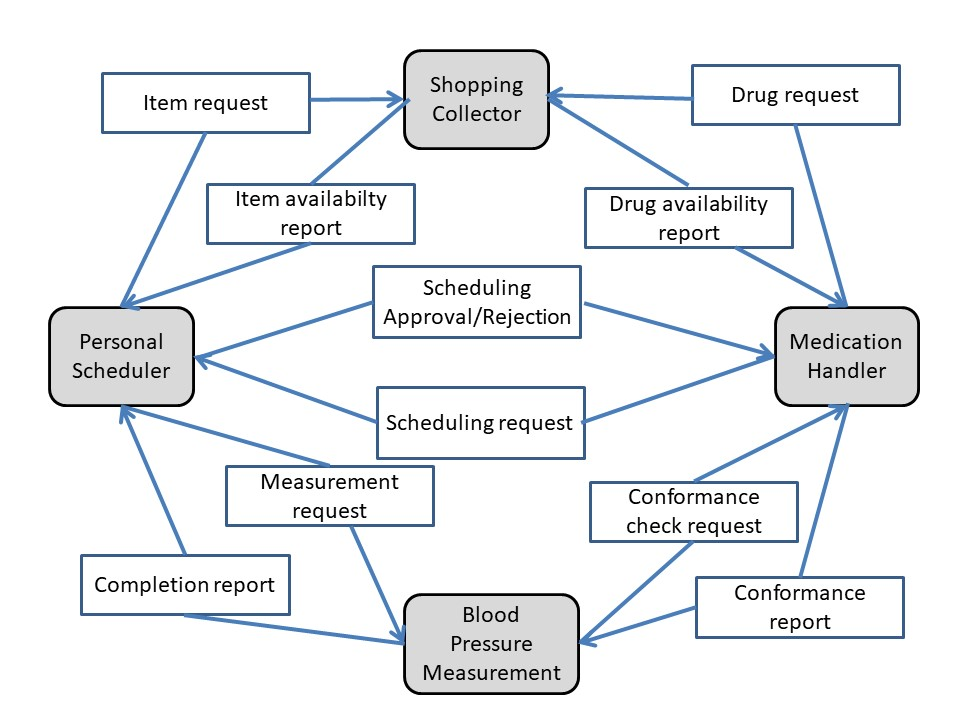
\includegraphics[width=0.6\linewidth] {Figures/Chapter5/Fog/homeCare.jpg}
	\caption[Example of home care support (SID)]{Example of home care support (SID)}
	\label{fig:homeCare}
\end{figure}


As usual Subject Behavior Diagrams (SBDs) provide a local view of the process from the perspective of individual subjects. 
\\
Given these capabilities, SoS Fog designs are characterized by (i) simple communication protocols (using SIDs for a process overview) and thus, (ii) standardized behavior structures (enabled by send-receive pairs between SBDs), which (iii) scale in terms of complexity and scope. 
\\
Subject-oriented Fog Computing (SFC) allows meeting ad-hoc and domain-specific requirements. As validated behavior specifications can be executed without further model transformation, stakeholders can guide the implementation of specification, representing domain-specific task flows, and make ad-hoc changes by replacing individual subject behavior specifications during runtime. Due to the distributed nature and loose coupling of subject-oriented representations, the ultimate stage of scalability could be reached through dynamic and situation-sensitive formation of edge systems.
\\
SFC structures SoS, e.g., when federating a blood pressure measurement device with a personal health scheduling systems, according to their communicating with each other. When these devices need to communicate directly with the cloud, e.g., as required in case of maintenance, or calling a specialist for medication, this link is encoded in the diagrams and executed during runtime after technical implementation. On the modeling layer the activity is a request sent to another subject, waiting until an answer is received, and processing the received answer. 

\subsubsection{Execution}
Once a Subject Behavior Diagram, e.g., for the Blood Pressure Measurement subject is instantiated, it has to be decided (i) whether a human or a digital device (organizational implementation) and (ii) which actual device is assigned to the subject, acting as technical subject carrier (technical implementation) (cf. \cite{Flei12}). Typical subjects as edge devices are smart devices, which can have Internet connectivity, including smart phones, tablets, laptops, healthcare devices, etc. The subject-oriented runtime engine \cite{article:StakeHolderCentered} is then a Fog Computing infrastructure providing low-latency virtualized services and is linked with the Cloud Computing infrastructure by the same subject interaction mechanism. As there can be a variety of edge devices, such a Fog Computing platform also needs to manage and control these devices (see also foglets described below). 
\\
Size, storage capacity, processing capabilities, and latency increase as we move closer to cloud computing. The subject-oriented Fog acts as an intermediate layer between the edge devices and the cloud. Edge devices request computing, storage and communication services from the Fog according to the subject-oriented communication scheme. The Fog provides local, low latency response to these requests and forwards relevant data for computationally intensive processing, long-term analytics and persistent storage over to the cloud. Figure[Fog Computing Architecture]{Fog Computing Architecture} provides a schematic visualization of this constellation, as it can be used for implementing the sample home healthcare support system.

\begin{figure}[htbp]
	\centering
	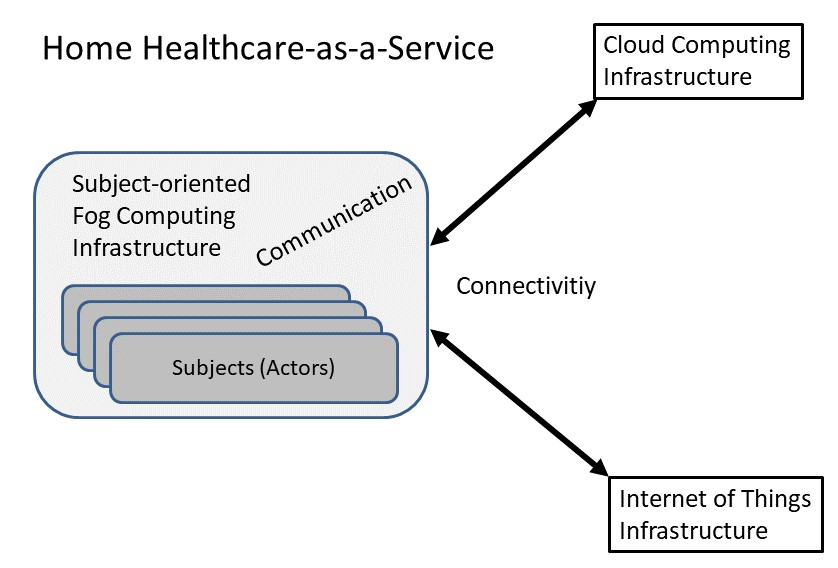
\includegraphics[width=0.6\linewidth] {Figures/Chapter5/Fog/FogArch.jpg}
	\caption[Fog Computing Architecture]{Fog Computing Architecture}
	\label{fig:FogArch}
\end{figure}

With respect to the home-healthcare example, a typical infrastructure comprises local devices and their interconnected services, such as linking the Blood Pressure Measurement to the Personal Scheduler. These subjects can be either linked to an IoT SoS, e.g., coupling several sensor systems, or to Cloud services, as for accessing public databases when checking reference or availability data, depending on the state of affairs in the home healthcare setting.
\\
Fog nodes are subject carriers representing resources including hardware (computing, networking and storage) capabilities. They provide ‘local’ real-time data processing capabilities, and, despite multi-tenancy, can execute applications in isolation to prevent unwanted interference from other processes. Policies to control service orchestration, filtering, and for adding security can be implemented dedicating a specific control subject, since the primary scheme of control is choreography.
\\
The approach scales, due to the decentralized management mechanisms allowing to setup, and configure a large number of devices in the Fog. In this context, subjects correspond to foglets (cf. \cite{article:OoTAnalytics}), i.e. software agents for each fog node, monitoring the state of the node and services. A subject can use abstraction tier APIs to monitor the state associated with (physical) devices and services deployed on this device. It analyses the entire information (encoded in an SBD), and delivers it to receivers linked through messages for further processing. These subjects can also perform lifecycle activities. As demanded by Vaquero et al. \cite{article:FiningwayFog}, SFC comprising a fog abstraction layer provides uniform programmable interfaces for resource control and management. 
\\
According to the S-BPM concepts, normalization can be used to abstract essential behavior patterns. For instance, in case Blood Pressure Management requires a machine-dependent procedure, its action behavior (performing functions) as a subject can in principle contain many internal functions which are performed in sequence, in order to accomplish an assigned task. In these sequences of internal functions, no sending and receiving nodes are included. Accordingly, extensive and therefore confusing behavior diagrams can be avoided. Since these sequences of internal functions are not important for communication, model representations can be simplified, and normalized behavior can lead to larger functions by hiding functional details. Actually, for the sake of understanding the home healthcare setting, the subjects shown in Figure \ref{fig:homeCare} have been normalized.
\\
In case the communication patterns are generalized, the process-network feature of S-BPM facilitates representation. For instance, when the Shopping Collector needs to collect sensor data from various storage devices, such as a refrigerator or a food isle, its communication requests and the respective replies can be denoted in a summative way. In SFC this feature helps representing mutually dependent processes, i.e., when subjects of a near-edge process communicate with subjects of other (near-edge) processes. As shown in Figure 5 the Home care near-edge process interacts with the Goods delivery process through the Personal Scheduler. In this case, the interaction is not further detailed, rather indicated through directed links. The same holds for the interaction between the Shopping Collector and the Medication Handler, which helps ensuring the quality of drug support in the Medicare process.

\begin{figure}[htbp]
	\centering
	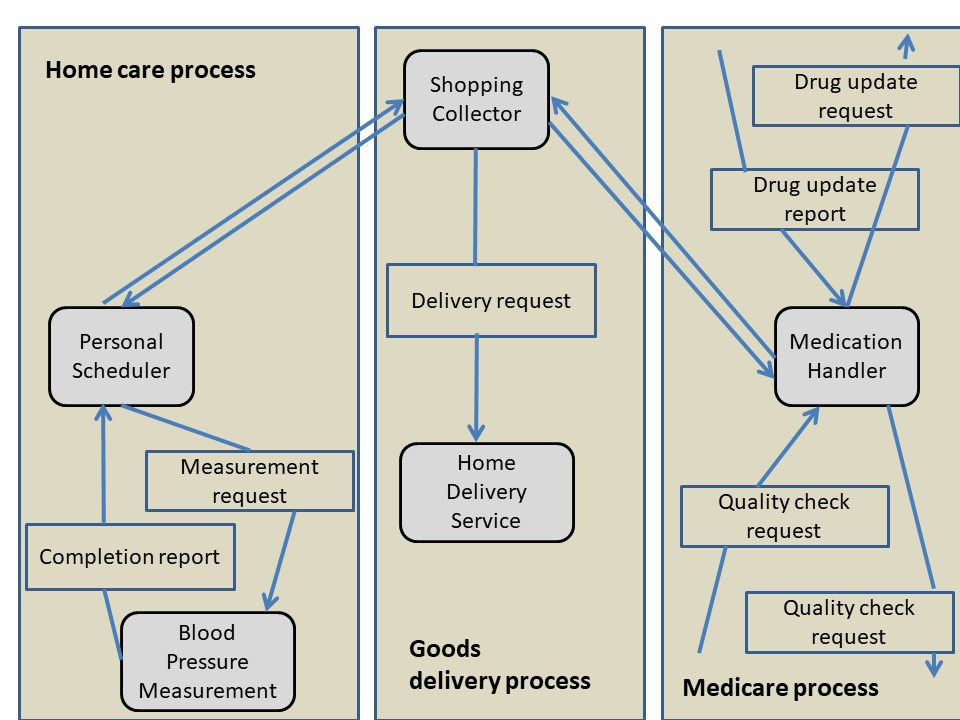
\includegraphics[width=0.6\linewidth] {Figures/Chapter5/Fog/InteractionHomeCare.jpg}
	\caption[Extended subject interaction diagram for the process ‘home care’]{Extended subject interaction diagram for the process 'home care'}
	\label{fig:InteractionHomeCare}
\end{figure}


For SFC implementation the open source engine UeberFlow \cite{DynamicPerspective} can be used. Hereby, SFC actions or tasks are ordered in the sequence as defined through SBDs and SIDs. The Workflow Specification of UeberFlow represents an entirely executable model of an application, given the subject actions and communication with others. It acts as container for so-called WorkflowUnits that are created for each subject, and captures all activities (WorkflowSteps). In addition, WorkflowUnit manages the data processed by the WorkflowSteps and its WorkflowFunctions. Consequently, Fog applications are executed through WorkflowSteps. 
\\
Thereby, the WorkflowFunctions are the most fine-grained units of execution in the UeberFlow Language meta-model, and define the actual execution logic of a WorkflowStep, its prerequisites and results. Once a step is triggered, a specific sequence of WorkflowFunctions is executed. The WorkflowFunctions can be one of 6 different types. For each of them an Actor has been implemented utilizing the Akka framework (http://akka.io/). Hence, an instance in UeberFlow is equivalent to all actor instances created in the context of this particular workflow instance. All of those actor instances are aggregated using the actor structuring and supervision mechanisms by defining a root actor representing the entire instance.

\subsection{Conclusion}
Fog Computing (FC) as a near-the-edge-computing paradigm has the potential to improve user support. When defined as a collection of various small distributed clouds deployed closer to the systems or devices at the edge of a communication network subject-oriented applications support 
\begin{list}{-}{spacing}
\item wide and dense geo-distribution due to their behavior abstraction, as e.g., required for home healthcare support systems, linking not only (medical) devices at home, but also medical infrastructure (physician, pharmacy, nursing services etc.) from the region
\item low or predictable latency due to the runtime concept of parallel processing 
\item cloud interplay of Fog nodes, due to separating specification from technical implementation which allows for processing data at different time scales, e.g., when monitoring body condition and supporting a patient treatment planning procedure 
\item multi-agencies choreography, loosening the need for orchestration, due to the inherent concept of choreography in subject-oriented architecting. Hence, Fog actors or subjects only need to be synchronized as tight as required, e.g., when a running monitor subject requires coordination with healthcare policy implementation at the same time
\item consistency, due to mapping all respective requirements to corresponding interaction patterns. Hence, demands and capabilities can be adjusted specifying message exchange patterns, in order to ensure overall consistent system states, either through subjects working in parallel, or through information distribution triggering further subject behavior.
\end{list}
Our future standardization effort will focus on including for networking information into the subject-oriented behavior abstractions, to enable modeling stakholder-specific settings according to their case-specific needs and available Fog actors. Once stakeholders are able to edit and validate the subject behavior models, they also can deal with organizational and technical implementation details, allowing them to adapt an entire application as System-of-System dynamically. Adaptation to new policies can be implemented in this way (cf. \cite{article:SecurityMgmt}), leading to more situation-sensitive Fog applications (cf. \cite{article:FogSimToolKit}). 



\section{Activity Based Costing}

CS: table refs are incorrect

\subsection{Basic Concepts}
\subsubsection{Process Controlling}
Process controlling has both a strategic and an operational dimension [cf. e.g. \cite{book:ProzesseSchmelzer}, p. 229 ff.]. We concentrate on methods and techniques for planning, designing and coordinating the supply of information necessary to allow continuous operational process controlling with key figures as indicated in the closed-loop approach to performance management (see lower part of figure \ref{fig:Approach-Performance} in \ref{sec:BAMinSubjectOrientation}). As operational process controlling aims for post-execution analysis of business process instances it can be complemented by Business Activity Monitoring (BAM) which, based on event processing concepts, observes instances during execution and sets alerts or triggers actions in real-time or near real-time according to the particular situations identified (cf. \cite{book:processmonitoring}, \cite{article:BlueprintEventDriven}).
\\
The major question is how to measure process performance. A typical parameter for the evaluation of process effectivity is customer satisfaction while process time, quality and cost and adherence to schedules are suitable to assess efficiency (cf. e.g. \cite{book:ProzesseSchmelzer} p. 229 ff.). As these parameters have high significance for the competitive position they are crucial for process controlling. While the assessment of customer satisfaction and maturity levels of processes usually are matters of periodic monitoring activities there might be other, more technical parameters needed to be watched permanently, like the response time of application systems. Those aspects are especially relevant if processes are extensively supported by IT.
\\
Figure \ref{fig:OpProcessCont} gives a conceptual overview of a key figure-based operational process controlling, split into continuous and periodic or occasional controlling activities, like it could be set up successively for the S-BPM approach.
The integrated collection and analysis of common managerial data allows for a cohesive evaluation and control in terms of process controlling [cf. \cite{book:ProzesseSchmelzer} p. 248 ff., 1 p. 385 ff., 7 p. 158 ff.]. It feeds back results to take decisions and actions, fostering a steadily growth of experience regarding the interdependencies between cost, quality and time (organizational learning).

\begin{figure}[htbp]
	\centering
	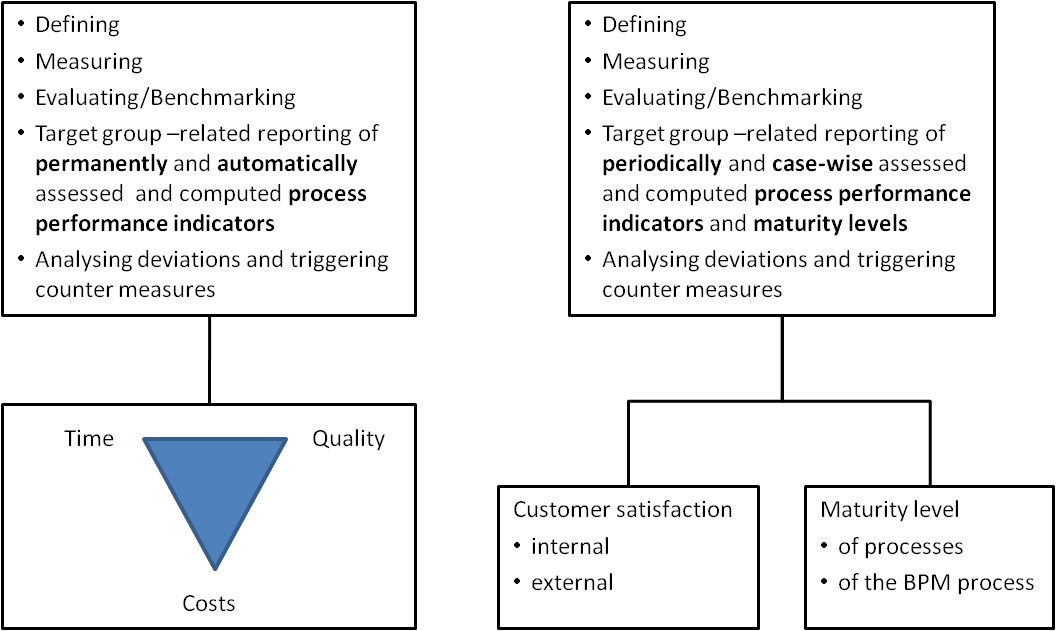
\includegraphics[width=0.6\linewidth] {Figures/Chapter5/ActivityBased/OpProcessCont.jpg}
	\caption[Operational Process Controlling]{Operational Process Controlling}
	\label{fig:OpProcessCont}
\end{figure}

In this section we focus on cost figures. Calculating them is more difficult than assessing those for time and quality. S-BPM allows determining cost figures for processes and process steps as well as for the occupation of cost centers and organizational units with little additional effort though. The reason is that S-BPM specifies subjects as actors in a process, their interaction and their assignment to elements of the organizational structure (organizational units, positions, roles). 
\\
The basic methodology to integrate such cost information into process controlling is Activity-Based Costing (ABC).


\subsubsection{Methodology of Activity-Based Costing}
The concept of Activity-Based Costing origins in the work of Miller and Vollmann \cite{article:HiddenFactory} and Cooper and Kaplan \cite{article:MeasureCost} and was established in the German-speaking community by Horvath und Mayer \cite{article:Prozesskosten}.
\\
ABC roots in a simple fact: producing and delivering a product or service involves many activities within cost centers and across boundaries of cost centers or functional areas, all causing costs. Major factors influencing these costs (cost drivers) usually are measures of the activity quantity, e.g. the number of purchasing orders being processed in procurement.
\\
\newline
\textbf{Step 1: Analysing activities}
\\
Starting point for ABC is an analysis of activities performed in the cost centers, using common methods like interviews, questionnaires, self-monitoring, third-party observation, document analysis or multi-moment recording. This analysis is essential for bordering cost center internal process steps and main processes running across cost center boundaries. Self-monitoring and multi-moment recording can bring up time standards for the execution of processes and their steps, but needs high effort. In order to ease the investigation of times, controllers instead often conduct interviews to find out what share of work force capacity the process steps occupy in a cost center.
The analysis results in a transparent, hierarchical process structure showing the assignment of activities to process steps, the assignment of process steps to cost centers and the aggregation of process steps to main processes (cf. figure \ref{fig:ProcessStruct} )

\begin{figure}[htbp]
	\centering
	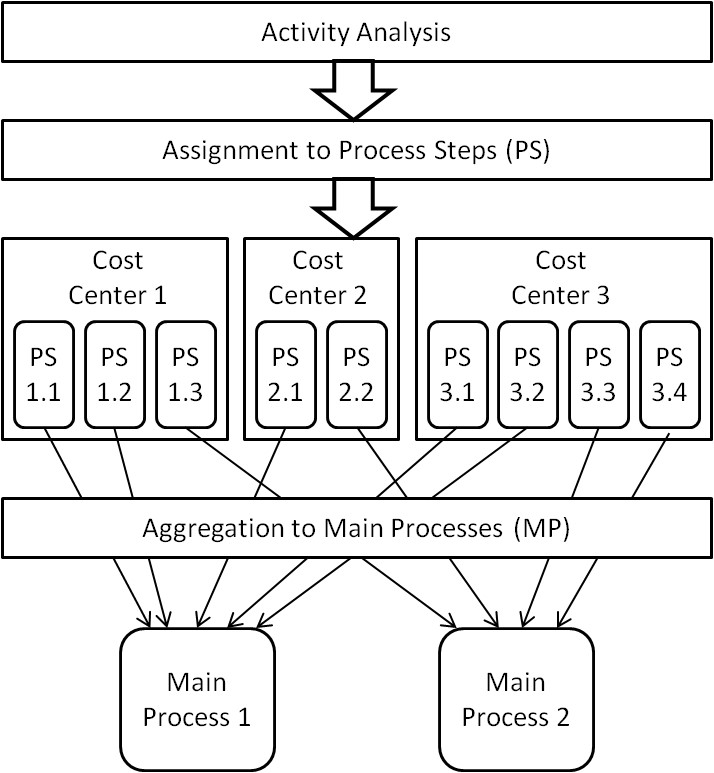
\includegraphics[width=0.6\linewidth] {Figures/Chapter5/ActivityBased/ProcessStruct.jpg}
	\caption[Process Structure]{Process Structure}
	\label{fig:ProcessStruct}
\end{figure}


This first step of Activity-Based Costing can be based on the results of the activity bundles analysis and modeling in S-BPM [6]. ABC-relevant information on subjects, their activities and the business objects being worked on are contained in the S-BPM process model (see section 2.3).
\\
\newline
\textbf{Step 2: Determining cost drivers}
\\
Horvath und Mayer differentiate between activity quantity induced (aqi) and activity quantity neutral (aqi) processes [9]. The latter (e.g. leading a department) cause costs independent from the activity quantity (e.g. the salary of the department leader). In activity quantity induced processes (e.g. purchasing goods) resource consumption and related costs vary with the activity quantity. Hereby process costs incurring depend on the number of cost drivers and there is need to determine measures for those as a second step in ABC. Cost drivers serve as an allocation base for resource utilization and thus also for causing costs.
\\
Cost drivers need to meet some requirements in order to make cost dependence transparent:
\begin{list}{-}{spacing}
	\item Process costs should, at least in the long term, vary with the activity quantity
	\item Cost driver values should be easy to assess and to understand.
	\item Input of resources should be approximately the same for all process instances, otherwise processes and cost drivers need to be further differentiated.
\end{list}

Usually ideas of what the major cost driver is already come up during the activity analysis and the activity quantity can be determined simultaneously then.
\\
\newline
\textbf{Step 3: Determining process costs}
\\
In practice it is often difficult to only assign the major cost driver to the main processes, because a main process can consist of process steps with different cost drivers not being proportionally related.
\\
In a given organizational and cost accounting context resources and costs are planned and actual costs are recorded on cost center level. This means planning and assessing process costs initially is also related to cost centers.
\\
Although theory suggests to plan process costs analytically and by cost type like in direct costing, practitioners prefer more simple concepts. One alternative is to only plan labor costs analytically and to allocate all other cost types proportionally. Another option would be to assign to the analyzed processes the capacities they consume and the related costs. In any case the accountants usually assume the labor cost to be the major cost element. Process costs then can be computed by multiplying a qualified estimate of the number of employees involved in the process by their average wage. If need be activity quantity neutral costs also can be passed on proportionally. In case there are more activity quantity induced costs with a significant extent they need to be considered in addition to labor costs. Even then the described procedure is still easy to handle.
\\
\newline
\textbf{Step 4: Determining process cost rate}
\\
In a last step, for the purpose of job order costing or product calculation, a simple division results in a process cost rate similar to the computation of a machine hour rate.
As shown Activity-Based Costing can be implemented in various ways. The identified problem of different cost drivers that cannot be aggregated can be solved by using time-related allocation bases \cite{article:Rechenzwecke} p. 23.
\\
The concrete process times can be computed if a workflow engine writes time stamps for begin and end events of the process steps. In order to have the engine processing a workflow at runtime, process activities must be assigned to concrete actors. Both kinds of information are needed for establishing ABC as elaborated in section \ref{section:ExampleABC}.


\subsection{BPM as Data Supplier}
Subject-oriented Business Process Management (S-BPM) focuses on the acting elements (actors) and their interactions as they drive a process. Its modeling notation includes all building blocks of a complete sentence in natural language as there are subject, predicate and object. The clear formal semantic of the underlying process algebra makes it possible to automatically generate code and makes subject-oriented process descriptions executable at a finger tip \cite{Flei12}, \cite{article:HMD-S-BPM}.
\\
Major parts of the model are subject interaction diagrams, describing the subjects involved in the process and the messages they exchange, and subject behavior diagrams, specifying subject activities as there are sending and receiving messages and other functions (e.g. manipulating business objects). The ladder means that at a time subjects can either be in a send, receive or functional state. 
Transforming the model into a workflow and integrating IT solutions (e.g. ERP functionality) to support particular activities is subject to the embedding of the process into IT. Assigning subjects to elements of the existing organizational structure (organizational units, positions, roles) being responsible for carrying out the activities as defined in the model, is called embedding the process (model) into the organization. Existing directory services based on Lightweight Directory Access Protocol (e.g. Active Directory) can ease the assignment of subjects to roles, groups and people as implemented in Metasonic Suite.
A process engine like Metasonic Flow interprets the model at runtime, instantiates process instances and controls their execution. According to the defined behavior the engine involves users and IT services or applications as subject representatives. It also controls the handling of business objects included the in subject behavior (creation, modification, deletion, exchange through messages). During execution the engine can capture many single pieces of data relevant for process controlling, especially by setting time stamps for state transitions and by counting instances. Examples are 

\begin{list}{-}{spacing}
\item begin time and end time of every single instance,
\item begin time and end time of the single steps within an instance or
\item number of instances of a certain process per time unit.
\end{list}
Using such raw data suitable software can compute key figures like
\begin{list}{-}{spacing}
\item waiting time of an instance from the moment it appeared in the in-box of an actor until he or she takes it out for processing (per case, on average) and
\item processing time from taking the instance out of the in-box until putting the result into the out-box (per case, on average).
\end{list}

This means the workflow system generates a valuable data basis for a meaningful Activity-Based Costing. This data needs to be categorized though and the key figures need to be defined precisely and unique in order to derive useful management information (see example in section \ref{section:ExampleABC}).

\subsubsection{Example for Estimating Process Costs in S-BPM} \label{section:ExampleABC}
Effective process controlling, allowing to turn such decisions into the right actions additionally requires information about cost dimensions in processes and cost-related consequences of processes for cost centers. Cost information enables monetary valuation of the enterprise performance as well as identifying weak points in operations and valuating their economic impact.
\\
We exemplify the determination of process costs using an order process. Figure \ref{fig:CalcPro} depicts the behavior diagram for the subject 'purchaser' enriched with some time information. These are times recorded as time stamps for state transitions by the process engine and stored in its event log \cite{article:SubProcessMon}. For clarity reasons in the figure \ref{fig:CalcPro} we only added time stamps for one state and just added the duration for the others.

\begin{figure}[htbp]
	\centering
	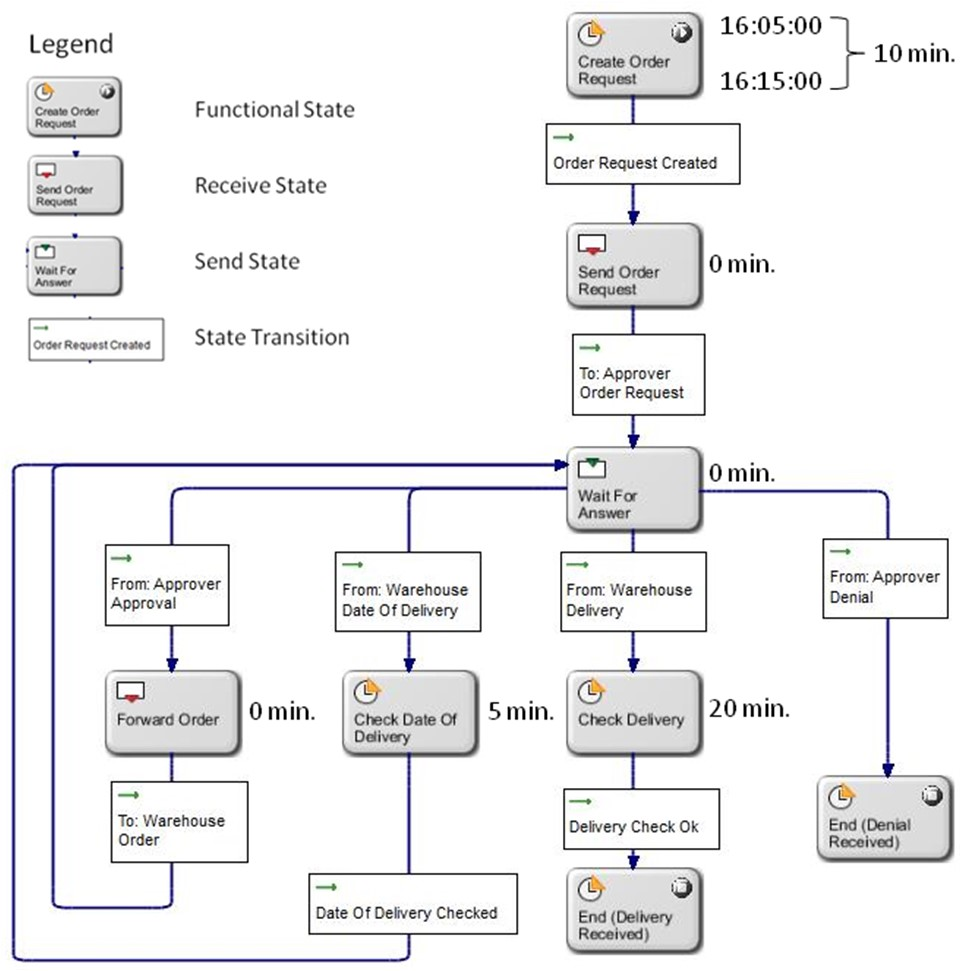
\includegraphics[width=0.6\linewidth] {Figures/Chapter5/ActivityBased/CalcPro.jpg}
	\caption[Calculating Processing Time of the Subject 'Purchaser']{Calculating Processing Time of the Subject 'Purchaser'}
	\label{fig:CalcPro}
\end{figure}


In the example the processing time of the subject 'purchaser' in case of the sunshine path (goods are on stock) can be computed by adding up the differences between start and end time of the functional states 'create order request' and 'check delivery'. The sunshine path sequence is as follows: After creating the request the purchaser sends it to the approver and then waits for an answer. If the request is denied the instance ends (right column in figure \ref{fig:CalcPro}). Otherwise the purchaser forwards the request to the warehouse (left column), waits for them to announce the delivery date and checks it (second to left). Finally he waits for the delivery and checks it after reception, before the instance comes to an end (third to left). As a simplification we assume the subject representatives to work permanently when performing functions (being in a functional state). We did not insert times for send and receive states because message exchange is considered to be accomplished electronically with no latency for sending, transmission and receiving. Applying this procedure to all subjects could lead to the result in table \ref{tab:procTime}.

\begin{table}[htbp]
	\centering
\begin{tabular}{|p{5.0 cm } |c|}
\hline
	\textbf{Subject} & Processing Time \\
	\hline
	\hline
	Purchaser & 35 min\\
	\hline
	Approver & 10 min \\
	\hline
	Warehouse & 30 min \\
	\hline
	Invoice Verification & 5 min \\
	\hline
	Accounting/book keeping & 5 min \\
	\hline
	Total & 85 min \\
	\hline
\end{tabular}
\caption{Processing times}
\label{tab:procTime}
\end{table}

For estimating the costs of the process we need an hourly or minute-related rate of wage for the people being assigned to the subjects. It is also possible to provide those values aggregated on group or role level. In Figure 5 we visualized how the subjects in our example are mapped to persons, while table \ref{tab:Hourly-wages-rate} gives an overview of the rates for the employees involved as subject representatives.

\begin{figure}[htbp]
	\centering
	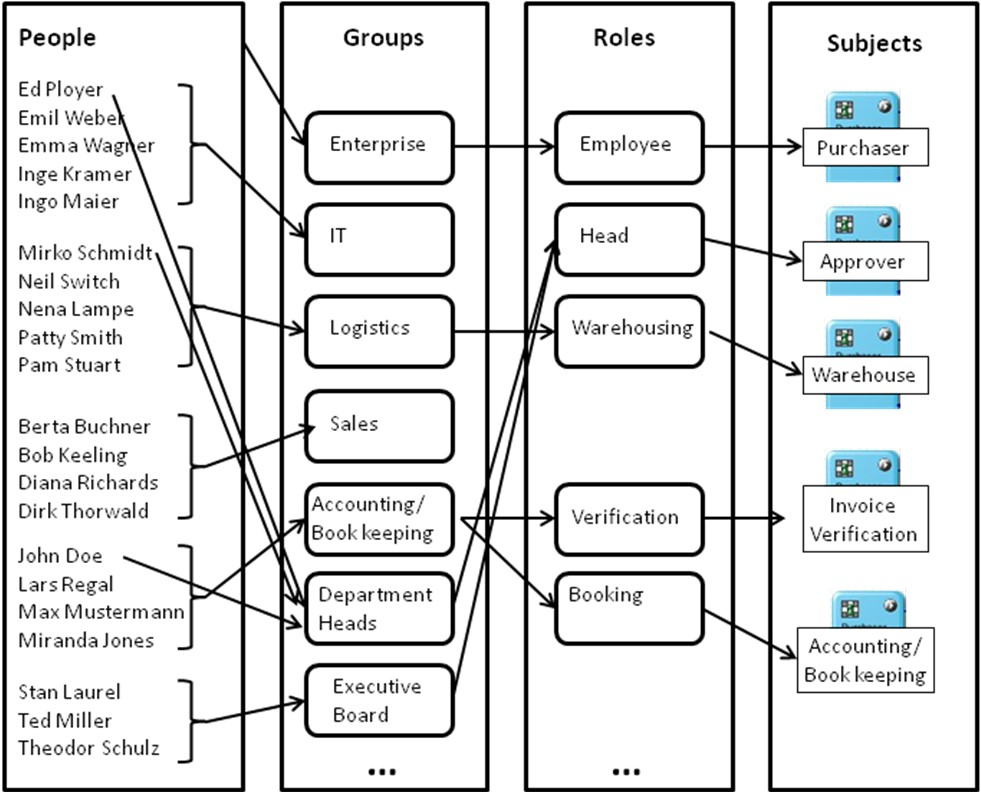
\includegraphics[width=0.6\linewidth] {Figures/Chapter5/ActivityBased/embedding.jpg}
	\caption[Embedding the Subjects into the Organization]{Embedding the Subjects into the Organization}
	\label{fig:Embedding}
\end{figure}

\begin{table}[htbp]
	\centering
	\begin{tabular}{|p{10.0 cm } |c|}
		\hline
		\textbf{Employee} & \textbf{Wage rate} \\
		\hline
		\hline
		Miller, Laurel, Schulz & 200 Euro/hour\\
		\hline
		Ployer, Schmidt, Doe, Keweling & 100 Euro/hour\\
		\hline
		Weber, Wagner, Kramer, Meier, Switch, Lampe, Smith, Stuart, Buchner, Richards, Thorwald, Regal, Mustermann, Jones & 50 Euro/hour\\
		\hline
	\end{tabular}
\label{tab:HourlyWages}
\caption{Hourly wages rate}
\end{table}



Having these time and wage values available it is a simple multiplication to determine the personnel-related process costs for every single instance (cf. table \ref{tab:ProcessCosts}). Considering a sufficient number of instances over a representative period of time allows computing a valid average cost value.

\begin{table}[htbp]
	\centering
	\begin{tabular}{|p{5.0 cm } |c|r|}
		\hline
		\textbf{Subject} & \textbf{Employee} & \textbf{Costs}\\
		\hline
		\hline
		Purchaser & Kramer & 35 Min. x 50 Euro/60 min.  =  29,17 Euro\\
		\hline
		Approver & Ployer & 10 Min. x 100 €/60 min. =  16,67 Euro\\
		\hline
		Warehouse & Lampe & 30 Min. x 50 €/60 min.  =  25,00 Euro\\
		\hline
		Invoice verification & Regal & 5 Min. x 50 €/60 min.    =    4,17 Euro\\
		\hline
		Accounting/Book keeping & Regal & 5 Min. x 50 €/60 min.    =    4,17 Euro\\
		\hline
		Total & & 79,18 Euro\\
		\hline
	\end{tabular}
\label{tab:ProcessCosts}
\caption{Personal Related Process Costs}
\end{table}

Assigning employees as subject representatives embeds the subjects into the organizational structure, because people belong to organizational units. As cost centers usually also are assigned to organizational units it is now possible to determine the costs of a process incurring in a certain cost center. From the cost center perspective it is also possible to see how its total costs are distributed over the processes and process steps it is involved in. Table \ref{tab:CostFig} shows examples for cost figures which can be computed.

\begin{table}[htbp]
	\centering
	\begin{tabular}{|p{3.0 cm } |p{10.0 cm }|}
		\hline
		\textbf{Key figure (Euro)} & \textbf{Computation (e.g. for 10 work days)}\\
		\hline
		\hline
		Process costs per process step/process & Multiply all processing times by the appropriate wage rate and aggregate the products over all instances occurring during the observation period\\
		\hline
		Process costs per cost center & Multiply all processing times incurring in the cost center by the appropriate wage rate and aggregate the products over all instances occurring during the observation period\\
		\hline
	\end{tabular}
\label{tab:CostFig}
\caption{Cost Figures}
\end{table}

As mentioned before key figures need to be defined carefully and precisely. A useful instrument helping to assure this are structured fact sheets being filled in with all necessary information \cite{book:KennzahlenIT}. Table \ref{tab:FactSgeet} depicts such a fact sheet created for our purposes \cite{book:MonitoringSubjekt}. A more formal structure can be found in \cite{article:ProcessPerfInd}.



\begin{table}[htbp]
	\centering
	\begin{tabular}{|p{3.0 cm } |p{10.0 cm }|}
		\hline
		\textbf{Attribute} & \textbf{Content}\\
		\hline
		\hline
		& \textbf{Characteristics}\\
		\hline
		Description & Average costs of a process activity for a certain period\\
		\hline
		To-be value/unit & tbd specifically (Euro)\\
		\hline
		Tolerance range/unit & tbd specifically (\%)\\
		\hline
		Escalation rule & In case of violation alert the process owner and start escalation process (tbd specifically)\\
		\hline
		Responsibility & Process Owner (tbd specifically)\\
		\hline
		\hline
		& \textbf{Measuring and Computing}\\
		\hline
		Measurement & Read time stamps written by Metasonic Flow, compute processing time as difference between time stamps for beginning and end, multiply processing time by hourly wage rate, divide product by number of completed instance\\
		\hline
		Algorithms & ∑ Processing time * hourly wage rate
					∑ completed instances\\
		\hline
		Data sources(general) & Tables in the database of Metasonic Suite:\newline
		RT\_PROCDESC, RT\_PROCINST, REC\_PARADESC, REC\_RECTRANS, UM\_USER\\
		\hline
		Data sources(specific) & Processing time:\newline
		\hspace*{4mm} \textbf{SELECT} TIMESTAMP1 \newline
		\hspace*{10mm} (\textbf{SELECT} STARTTIME \newline
		\hspace*{10mm} \textbf{FROM} RT\_PROCINST \newline
		\hspace*{10mm} \textbf{WHERE} RT\_PROCDESC = \textit{process} \newline
		\hspace*{10mm} \textbf{AND} ID = \textit{instance} \newline
		\hspace*{4mm}\textbf{FROM} REC\_RECTRANS \newline
		\hspace*{4mm}\textbf{WHERE} RT\_STDESC = \textit{state} \newline
		\hspace*{4mm}\textbf{AND} RT\_PROCINST = \textit{instance} \newline
		Hourly wage rate: UM\_USER (manually enriched by hourly wage rates) \newline
		Completed instances: see separate fact sheet\\
		\hline
		Frequency & weekly\\
		\hline
		\hline
		& \textbf{Presentation} \\
		\hline
		Addressees & Process Owner, Middle Management, Accountants (tbd specifically)\\
		\hline
		Presentation & As-is value and to-be value in combination with a sparkline showing the historical development, deviation from to-be value in \%\\
		\hline
		Archiving & Stored in additional database table, linked with RT\_PROCDESC\\
		\hline
	\end{tabular}
\label{tab:FactSgeet}
\caption{Fact Sheet for the Key Figure 'Average costs of a process activity'}
\end{table}

\subsection{Conclusion and Future Work}
With the example in chapter 3 we could show that it is relatively easy to integrate cost information into S-BPM. Focusing on personnel costs as suggested avoids the problematic proportioning of costs and therefore is particularly suited for people-intensive areas with a high degree of indirect costs as it is characteristic for services.
A more detailed investigation of how the implementation of Activity-Based Costing can benefit from a preceding S-BPM implementation seems to be promising. Exploiting the conceptual particularities coming with and the data collected by S-BPM seems to bear considerable potential of savings when introducing ABC. Processes are defined and modeled and as-is process quantities per period are available as well as the distribution of the overall capacity of the cost centers over the process steps. These parameters allow determining a standard time for processes which lays the ground for planning process costs.
Next steps could be to extend the example by determining and specifying more key figures and testing them with representative numbers of instances of different processes. Learning from this could help to further elaborate the ABC concept for S-BPM.
References

